% ****** Start of file apssamp.tex ******
%
%   This file is part of the APS files in the REVTeX 4.1 distribution.
%   Version 4.1r of REVTeX, August 2010
%
%   Copyright (c) 2009, 2010 The American Physical Society.
%
%   See the REVTeX 4 README file for restrictions and more information.
%
% TeX'ing this file requires that you have AMS-LaTeX 2.0 installed
% as well as the rest of the prerequisites for REVTeX 4.1
%
% See the REVTeX 4 README file
% It also requires running BibTeX. The commands are as follows:
%
%  1)  latex apssamp.tex
%  2)  bibtex apssamp
%  3)  latex apssamp.tex
%  4)  latex apssamp.tex
%
\documentclass[%
 reprint,
%superscriptaddress,
%groupedaddress,
%unsortedaddress,
%runinaddress,
%frontmatterverbose, 
%preprint,
%showpacs,preprintnumbers,
%nofootinbib,
%nobibnotes,
%bibnotes,
 amsmath,amssymb,
 aps,
%%pra,
prl,
%rmp,
%prstab,
%prstper,
%floatfix,
]{revtex4-1}

\usepackage{graphicx}% Include figure files
\usepackage{dcolumn}% Align table columns on decimal point
\usepackage{bm}% bold math
\usepackage[colorlinks=true, citecolor=red, linkcolor=blue, urlcolor=black]{hyperref}% add hypertext capabilities
%\usepackage[mathlines]{lineno}% Enable numbering of text and display math
%\linenumbers\relax % Commence numbering lines

%\usepackage[showframe,%Uncomment any one of the following lines to test 
%%scale=0.7, marginratio={1:1, 2:3}, ignoreall,% default settings
%%text={7in,10in},centering,
%%margin=1.5in,
%%total={6.5in,8.75in}, top=1.2in, left=0.9in, includefoot,
%%height=10in,a5paper,hmargin={3cm,0.8in},
%]{geometry}

\usepackage{pgffor}

\usepackage{tikz}
\newcommand{\tikzcircle}[2][red,fill=red]{\tikz[baseline=-0.5ex]\draw[#1,radius=#2] (0,0) circle ;}%
\newcommand{\site}{\tikzcircle[fill=none]{2pt}}
\newcommand{\magnon}{\tikzcircle[fill=red]{2pt}}
\newcommand{\hole}{\tikzcircle[fill=blue]{2pt}}

\def\d{{\textit{d}}}
\newcommand*{\field}[1]{\mathbb{#1}}%

\newcommand{\bra}[1]{\langle#1\rvert}
\newcommand{\ket}[1]{\lvert#1\rangle}
\newcommand{\mean}[1]{\langle#1\rangle}

\newcommand{\Bra}[1]{\left\langle#1\left\rvert}
\newcommand{\Ket}[1]{\right\lvert#1\right\rangle}

\newcommand{\AFA}{\ket{\downarrow\uparrow\downarrow\uparrow\downarrow\uparrow\hdots}}
\newcommand{\AFB}{\ket{\uparrow\downarrow\uparrow\downarrow\uparrow\downarrow\hdots}}

\newcommand{\FMA}{\ket{\uparrow\uparrow\uparrow\uparrow\uparrow\uparrow\hdots}}
\newcommand{\FMB}{\ket{\downarrow\downarrow\downarrow\downarrow\downarrow\downarrow\hdots}}

\def\tj{{$t$--$J$}}
\def\tjz{{$t$--$J^z$}}
\def\tjlam{{$t$--$J$--$\lambda$}}
\def\square{{$\mathbb{Z}^2$}}

\begin{document}

%\preprint{APS/433-SAW}

\title{
The fate of the spin polaron in the 1D antiferromagnets
}

\author{Piotr Wrzosek$^1$}
\email{Piotr.Wrzosek@fuw.edu.pl}
\author{Adam K\l{}osi\'nski$^1$}
\author{Yao Wang$^2$}
\author{Mona Berciu$^3$}
\author{Cli\`o Efthimia Agrapidis$^1$}
\author{Krzysztof Wohlfeld$^1$}
 
\affiliation{%
$^1$Institute of Theoretical Physics, Faculty of Physics, University of Warsaw, Pasteura 5, PL-02093 Warsaw, Poland
}%

\affiliation{%
$^2$Department of Physics and Astronomy, Clemson University, Clemson, South Carolina 29631, USA
}%

\affiliation{%
$^3$Dept. of Physics \& Astronomy, University of British Columbia, Vancouver, BC, Canada
and Quantum Matter Institute, University of British Columbia, Vancouver, BC, Canada
}%

\date{\today}% It is always \today, today,
             %  but any date may be explicitly specified

\begin{abstract}
The stability of the spin polaron quasiparticle, well established in studies of a single hole in the 2D antiferromagnets, is investigated in the 1D antiferromagnets using a $t$--$J$ model. We  perform an exact slave fermion transformation to the holon-magnon basis, and  diagonalize numerically the resulting model in the presence of a single hole. We prove that the spin polaron is stable for any strength of the magnon-magnon interactions {\it except} for the unique value of the SU(2)-symmetric 1D $t$--$J$ model. Fine-tuning to this unique value is extremely unlikely to occur in {\it quasi}-1D antiferromagnets, therefore the spin polaron is the stable quasiparticle of real 1D materials. Our results lead to a new interpretation of the ARPES spectra of {\it quasi}-1D antiferromagnets in the spin polaron language.
%
\end{abstract}

\pacs{Valid PACS appear here}% PACS, the Physics and Astronomy
                             % Classification Scheme.
%\keywords{Suggested keywords}%Use showkeys class option if keyword
                              %display desired
\maketitle


\def\L{28}



{\it Introduction}  A central problem in the study of strongly correlated systems  is to understand the differences between quantum many-body systems that have stable low-energy quasiparticles, and those that do not~\cite{Khomskii2010, Zaanen2019, Kumar2021, Lauchli2004, Ver19}. A famous example, which we revisit, relates to expected fundamental differences between the low-energy physics of 1D and 2D antiferromagnets doped with a single hole. The widely accepted paradigm is that in a 2D antiferromagnet, the hole is dressed with collective 2D spin excitations (magnons) and together they form a spin polaron quasiparticle~\cite{Bul68, Sch88, Mar91, Gru18, Chi18, Koepsell2019, Koepsell2021, Wang2021, Bohrdt2021_01}, whereas in 1D, the spin polaron is unstable to splitting into an elementary 1D spin excitation (spinon) and a spinless hole (holon), a phenomenon called  spin-charge separation~\cite{Lieb1968, Voi95, Kim96, Kim1997, Fujisawa1999, Poilblanc2006, Koitzsch2006, Kim06, Jayadev2020}. 

The paradigmatic explanation for this difference  relies on the fact that spinons (magnons) are well-defined collective excitations in 1D (2D) antiferromagnets~\cite{Khomskii2010}. Because our goal is to understand the \textit{intrinsic} origin of the different single hole behaviour in 1D and 2D antiferromagnets, we have to use the same language to describe both cases. As the 1D case is always easier to study~\cite{Giamarchi2003}, we choose to recast the 1D problem using the 2D magnon language so that we can answer the question: what is the fate of the spin polaron in the 1D antiferromagnets?

In this Letter we answer this question by: (i) developing a novel  numerical simulation of the $t$--$J$ model in the magnon-holon basis~\cite{Mar91}, and (ii) performing a detailed finite size scaling of the quasiparticle properties. We show that the spin polaron quasiparticle is destroyed in the ground state of the 1D antiferromagnet with a single hole {\it only} when the magnon-magnon interactions are precisely tuned to the unique value dictated by the 1D $t$--$J$ model. 
For any other value of the magnon-magnon interaction, whether stronger or weaker than this critical value~\footnote{Interestingly, this situation is distinct from the one reported in~\cite{Ver19}, in which interactions {\it support} the stability of a quasiparticle.}, the spin polaron is the stable quasiparticle of the 1D antiferromagnet. 
In particular, we show that the staggered magnetic field present in {\it quasi}-1D antiferromagnets of real materials~\cite{Kojima1997, Matsuda1997, Lake2005}
disrupts this fine balance between the on-site magnon energy and the magnon-magnon interaction of the 1D $t$--$J$ model.
This makes the spin polaron quasiparticle stable in the {\it quasi}-1D cuprates and leads to the interpretation of the ARPES spectra~\cite{Sobota2021} 
of {\it quasi}-1D cuprates~\cite{Kim96, Kim1997, Fujisawa1999, Koitzsch2006, Kim06} in the spin polaron language. Our results show an unexpected, impressive robustness of the spin polaron picture in the {\it quasi}-1D antiferromagnets, proving that the accepted spin-charge separation paradigm is in fact an exception~\cite{Bonca1992, Greiter2002,  Schmidt2003, Smakov2007, Lake2010, Yang2022}, not the rule~\cite{Giamarchi2003}. The obtained results have important consequences reaching beyond condensed matter, {\it inter alia} in the interpretation of cold atom experiments~\cite{Bohrdt2021, Koepsell2021}.

{\it Model and methods}
The Hamiltonian of the standard model of a doped antiferromagnetic chain, the $t$--$J$ model~\cite{Chao1978}, reads,
\begin{equation} \label{eq:H}
    \mathcal{H} = -t\!\!\sum_{\mean{i,j},\sigma}\!\! \left( \tilde{c}_{i,\sigma}^\dag \tilde{c}_{j,\sigma}\! +\! \text{h.c.}\right) + J\!\sum_{\mean{i,j}}\!\!\left(\mathbf S_i \! \cdot\! \mathbf S_j\! -\! \frac{1}{4}\tilde{n}_i\tilde{n}_j \!\right)\!,
\end{equation}
where $\tilde{c}_{i,\sigma}^\dag = c_{i,\sigma}^\dag (1 - n_{i,\bar{\sigma}})$ creates the electron only on unoccupied site, $n_{i,\sigma} = c_{i,\sigma}^\dag c_{i,\sigma}$ and $\tilde{n}_i = \sum_{\sigma}\tilde{c}_{i,\sigma}^\dag\tilde{c}_{i,\sigma}$. Moreover, $\mathbf S_i$ are spin-1/2 Heisenberg operators at site $i$. We rewrite the model in terms of bosonic magnon $a_i$ and fermionic holon $h_i$ operators by means of Holstein-Primakoff (HP) and slave-fermion transformations, respectively~\cite{Mar91}. 
This leads to the following form of the $t$--$J$-like Hamiltonian:
\begin{align}
\label{eq:model}
\mathcal{H} =&~t \sum_{\mean{i,j}} \left[ h_i^\dag h_j
\left( a_i + a_j^\dag P_i \right) + h_j^\dag h_i \left( a_j + a_i^\dag
P_j \right) \right] \nonumber \\ 
+& \frac{J}{2} \sum_{\mean{i,j}} \left[ a_i
a_j + a_i^\dag a_j^\dag P_i P_j
+ a_i^\dag a_i + a_j^\dag a_j -2 \lambda a_i^\dag a_i a_j^\dag a_j
\right] \nonumber \\
+& \frac{J}{2} \sum_{\mean{i,j}} \left[
h_i^\dag h_i P_j + h_j^\dag h_j P_i - h_i^\dag h_i h_j^\dag h_j \right],
\end{align}
where $P_i \equiv 1-a_i^\dag a_i$~\cite{Kon21}.
The above model with $\lambda=1$ follows from the \textit{exact} mapping of the $t$--$J$ model. However, we also discuss results with $\lambda\ne 1$ so as to understand the effects of tuning the strength of the magnon-magnon interaction. We solve the above model numerically using Lanczos algorithm~\cite{KrylovKit}.

\begin{figure}[t!]
    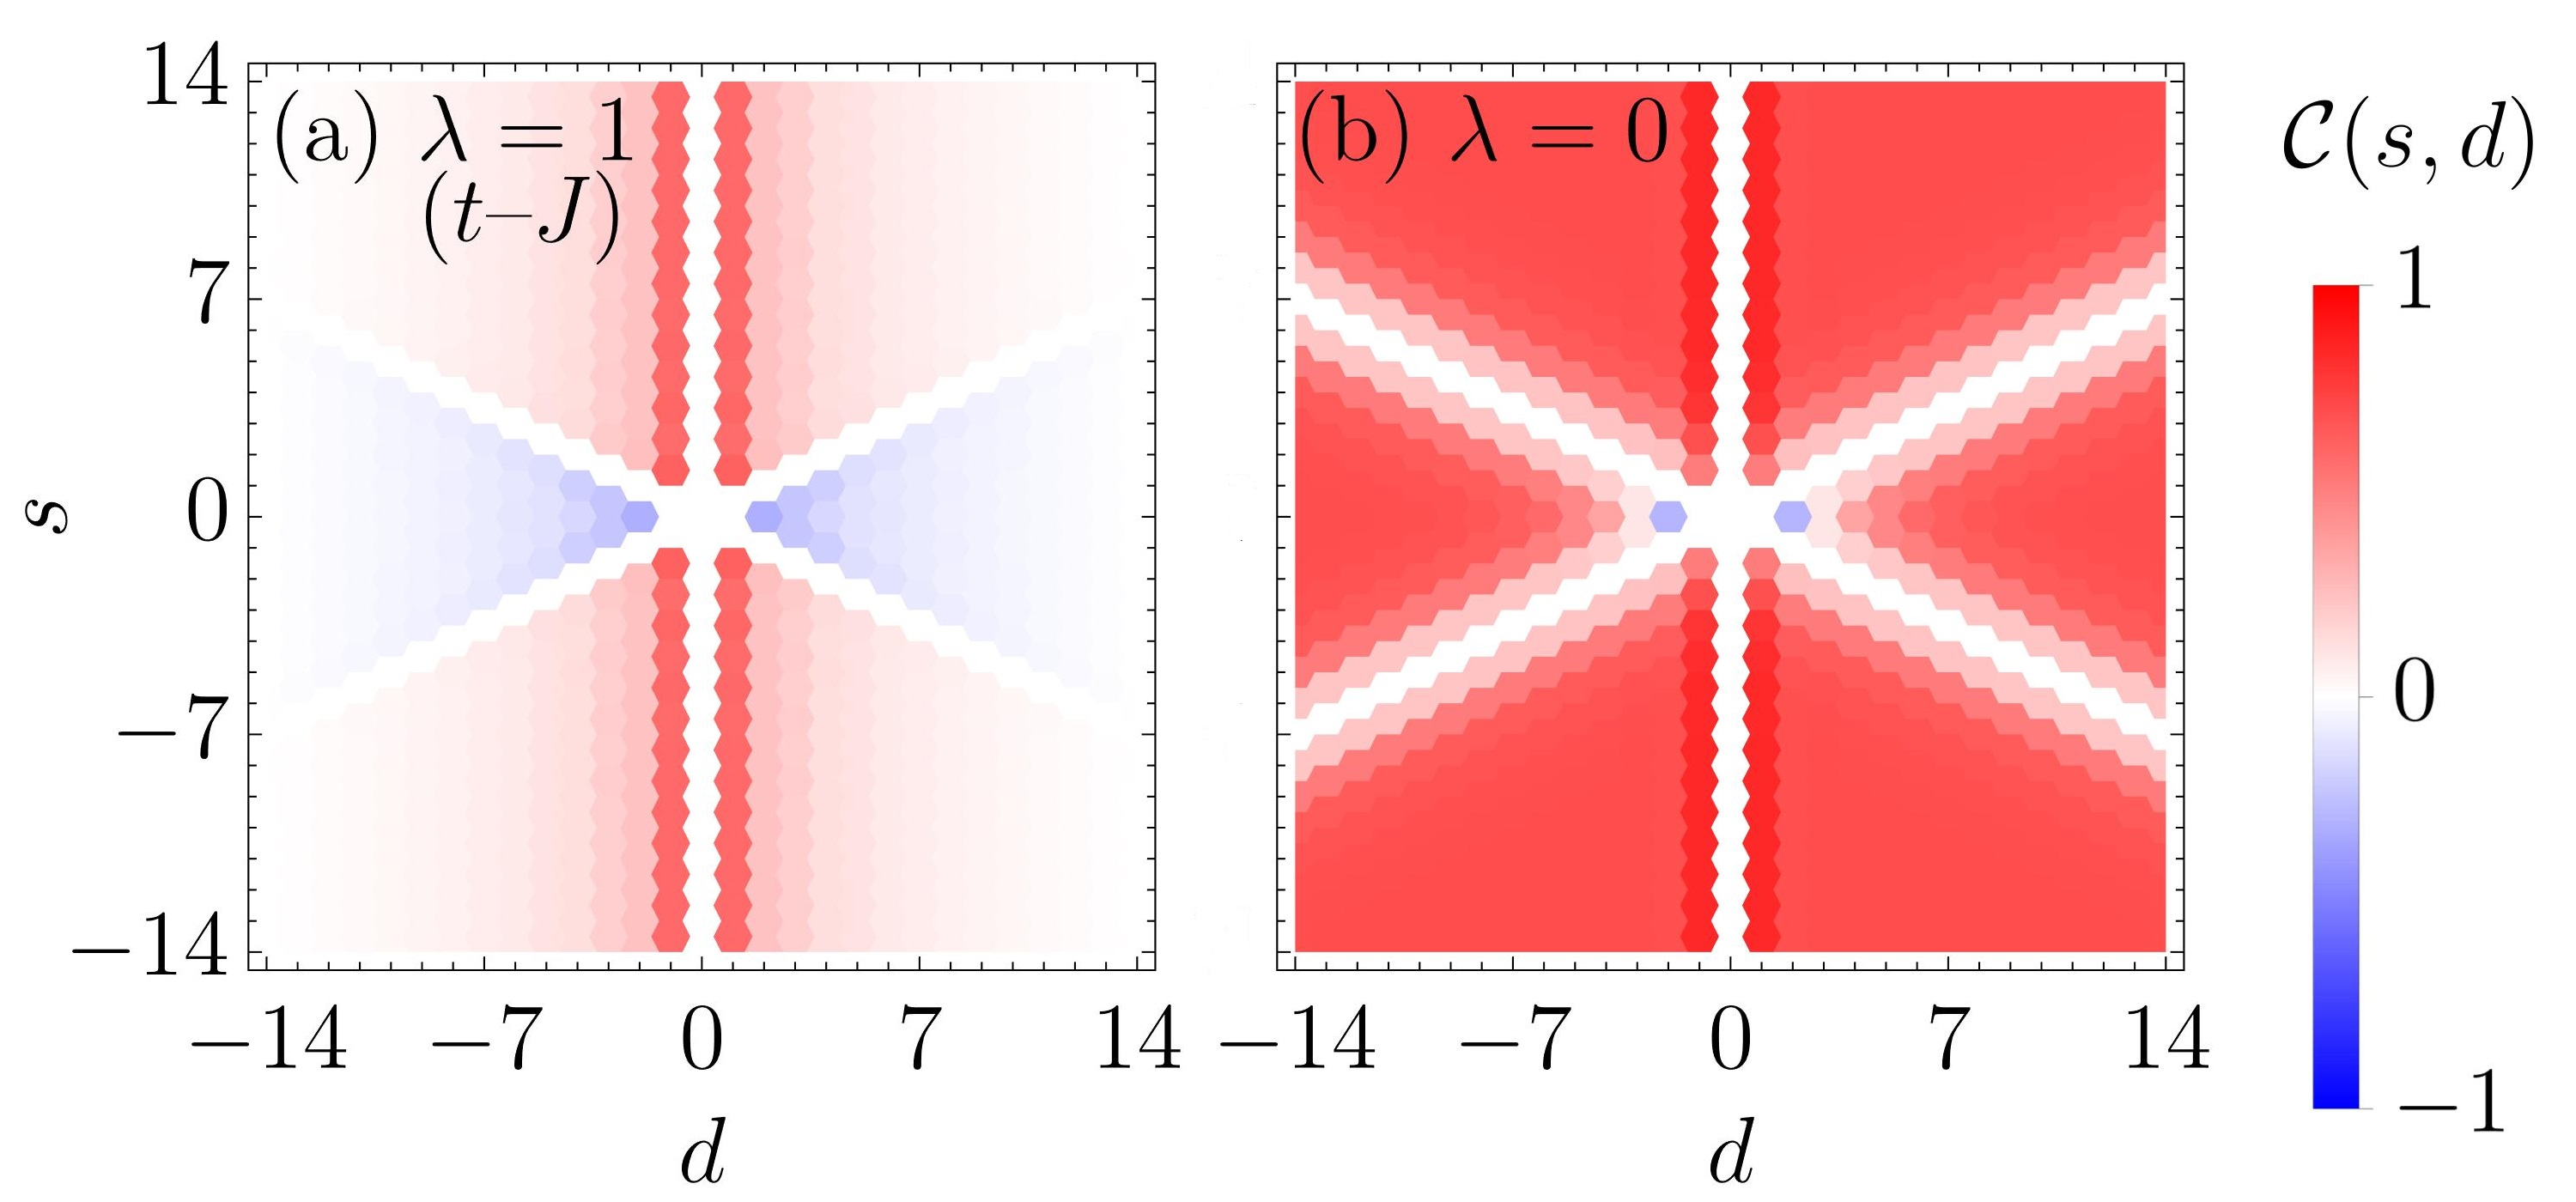
\includegraphics[width=\columnwidth]
    {fig_1.jpg}
  \caption{Magnetic properties of the 1D $t$--$J$ model ground state with a single hole as probed by the hole-spin correlation function $\mathcal{C}(s, d)$: (a) with  magnon-magnon interactions `correctly' included, i.e. with their value as in the 1D $t$--$J$ model [model \eqref{eq:model} with $\lambda = 1$], (b) without the magnon-magnon interactions [model \eqref{eq:model} with $\lambda = 0$]. Calculation performed on the \L~sites long periodic chain using exact diagonalization and for $J=0.4t$, see text for further details.
}
\label{fig:correlator}
\end{figure}

{\it Results: ground state} We begin by studying the influence of the magnon-magnon interactions on the magnetic properties of the ground state of the 1D $t$--$J$ model with a single hole, cf. Fig.~\ref{fig:correlator}(a) vs. Fig.~\ref{fig:correlator}(b). To this end we choose the following 
three-point correlation function 
\begin{align}
\mathcal{C} (s,d) = (-1)^{d} 4 L \big{\langle} S_0^z  (1- \tilde n_{s+d/2})   S_{d}^z \big{\rangle}.
\end{align}
Here $d$ denotes the distance between the two spins, $s$ is the distance of the hole from the center of mass of the two spins and $L$ is the number of sites. As shown in Ref.~\onlinecite{Hilker2017} this `hole-spins' correlator tracks
the sign changes of the spin correlations due to the presence of the hole
and hence can be used to verify whether  spin-charge separation occurs in the system. Indeed, for the 1D $t$--$J$ model, i.e. once the parameter governing magnon-magnon attraction is tuned to the value of $\lambda = 1$ in model \eqref{eq:model}, we fully recover the result of Ref.~\onlinecite{Hilker2017} and 
as shown in Fig.~\ref{fig:correlator}(a), the positive and negative correlation regimes are separated and extend to the largest accessible distance, reflecting the spin-charge separation nature.
This contrasts with the hole-spins correlator calculated for model \eqref{eq:model} with $\lambda =0$. Once the magnon-magnon interactions are switched off, cf. Fig.~\ref{fig:correlator}(b),
the negative correlation is restricted to a very small regime with small $d$, indicating that the spinon and holon cannot be arbitrarily far apart.
This sign structure of the hole-spins correlator is a signature of the spin polaron.

\begin{figure}[t!]
    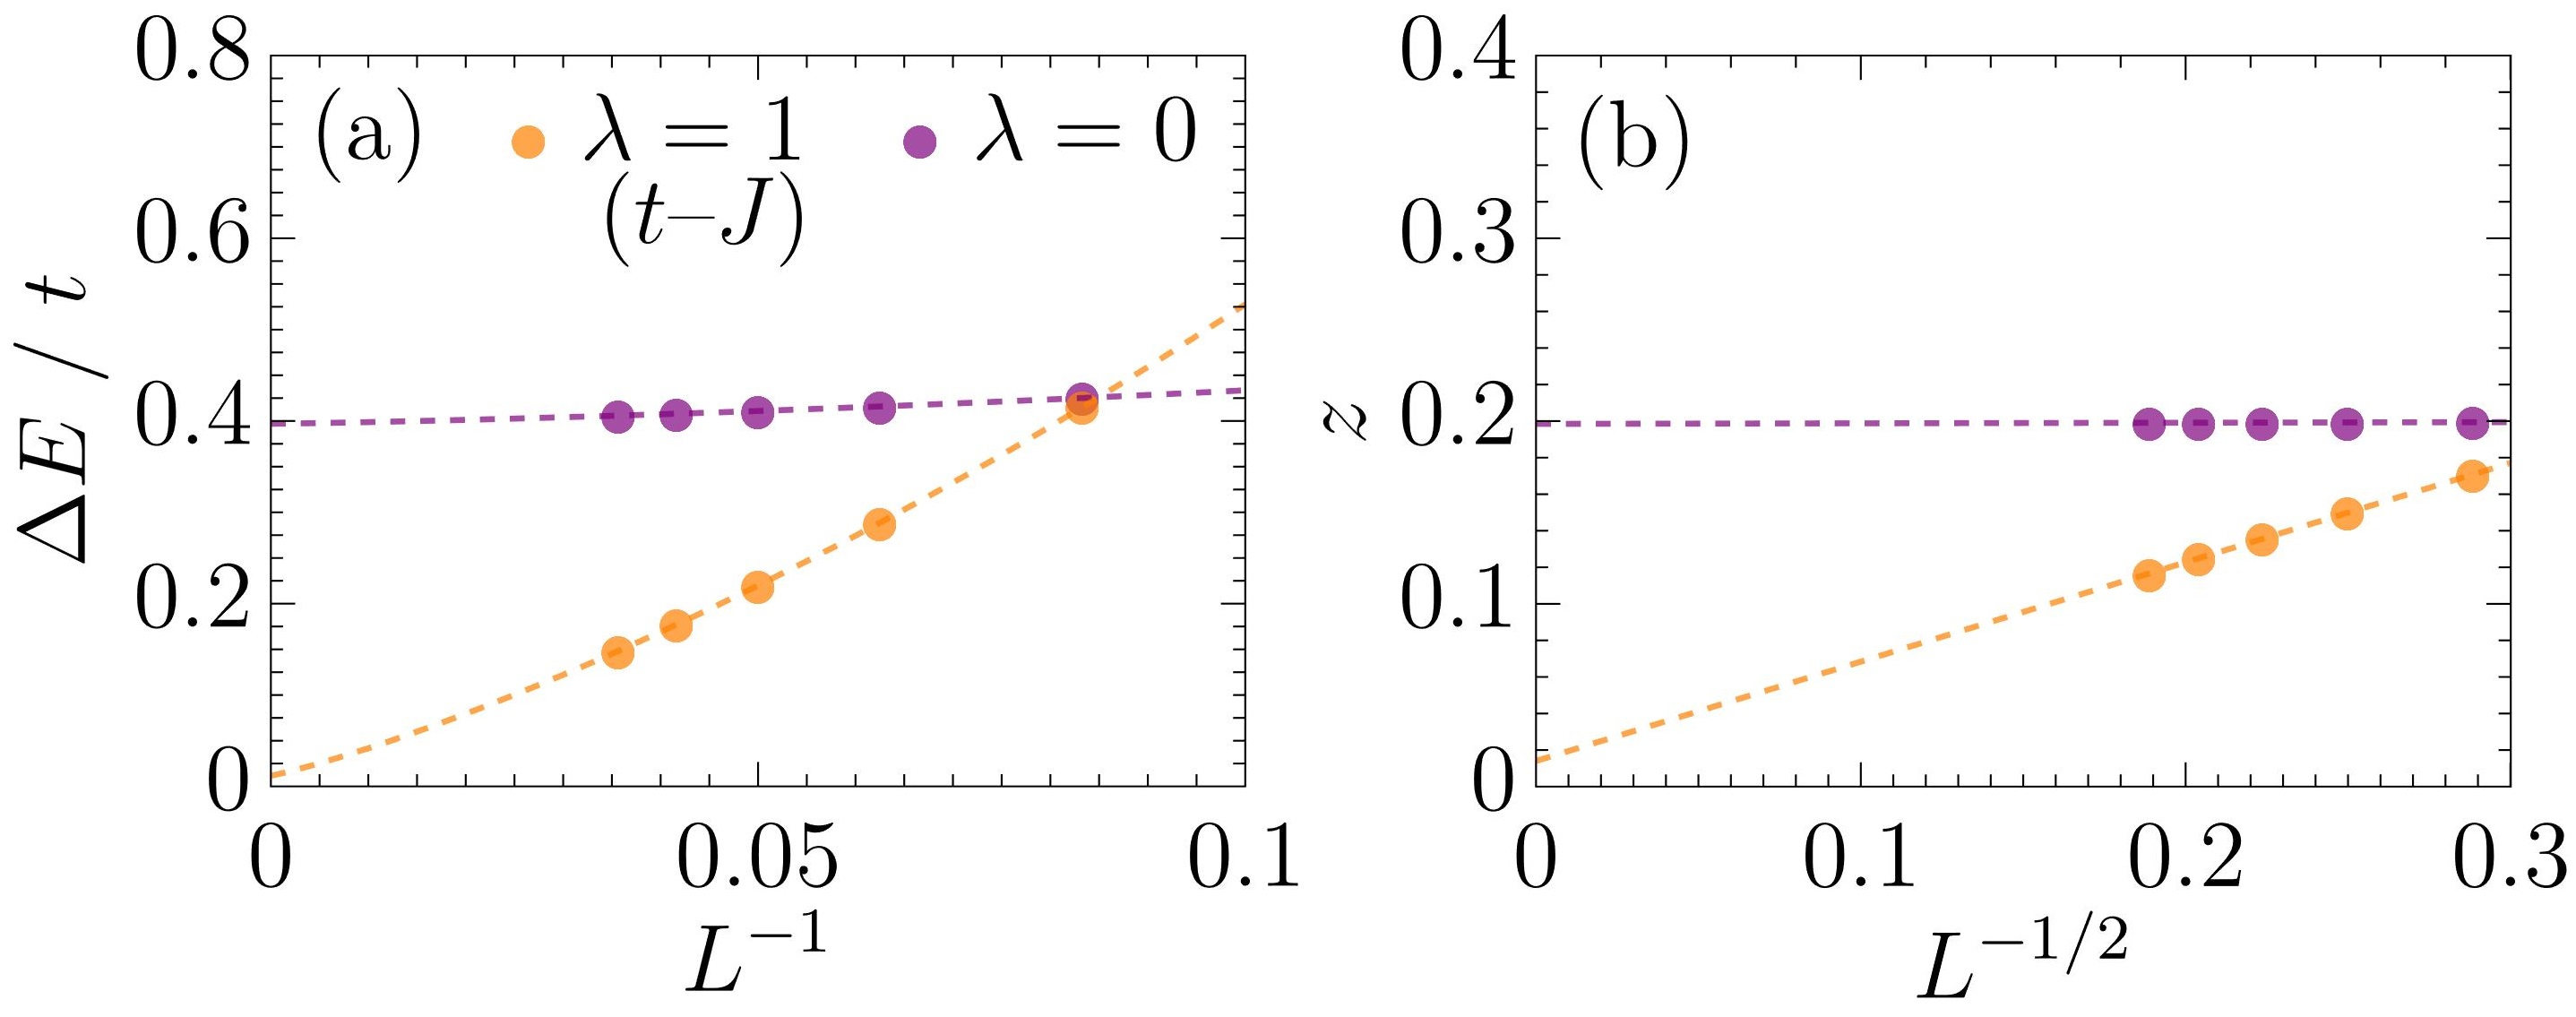
\includegraphics[width=\columnwidth]
    {fig_2.jpg}
  \caption{Dependence of the quasiparticle properties of the ground state of the 1D $t$--$J$ model with a single hole on the system size $L$: (a) the energy difference $\Delta E$ between the ground state and the first excited state at the same pseudomentum; (b) the quasiparticle spectral weight $z$, i.e. the overlap between the ground state and the `Bloch wave' single particle state. Results with the magnon-magnon interactions correctly included [$\lambda=1$ in \eqref{eq:model}] and without the magnon-magnon interactions [$\lambda=0$ in \eqref{eq:model}]
%
are shown using magenta and orange symbols, respectively.
Calculation performed on chains of length $L$ and with  $J = 0.4t$; see text for details on the functions fitted to the data.
}
\label{fig:scaling}
\end{figure}

To irrevocably verify the stability of the spin polaron in a 1D antiferromagnet, 
we perform a finite-size scaling analysis of the two crucial quantities defining the quasiparticle properties of the ground state: (i) the energy gap ($\Delta E$) between the ground and first excited states (at the same pseudomomentum), and (ii) the quasiparticle spectral weight ($z$), i.e. the overlap between the ground state and the corresponding `Bloch wave’ single particle state. 

To obtain the value of the energy gap $\Delta E$ in the thermodynamic limit we assume that $\Delta E$ scales linearly, up to a small logarithmic correction, as a function of the inverse system size $1/L$~\footnote{This is due to: (i) the mapping of the problem of a single hole in the $t$--$J$ model onto a Heisenberg model with the shifted boundaries, cf.~\cite{Sorella1998}, and (ii) the energy gaps scaling in the latter model as $1/L$
with a small logarithmic correction, cf.~\cite{Haas1998}.} The finite size scaling analysis on the $t$--$J$ model ($\lambda=1$) unambiguously shows that the energy gap quickly decreases with increasing system size and we obtain 
a vanishing $\Delta E$ in the thermodynamic limit within $10^{-2}t$ accuracy,
cf. Fig.~\ref{fig:scaling}(a).
This scaling behavior is consistent with the appearance of a low-energy continuum, which has been well demonstrated by exact diagonalisation of the $t$--$J$~model.
This result for the $t$--$J$ model ($\lambda =1$) stands in stark contrast with the one obtained for the case without magnon-magnon interactions ($\lambda=0$); in that case the energy gap $\Delta E$ scales to a finite value ($\sim 0.4 t$ for $J=0.4t$), cf. Fig.~\ref{fig:scaling}(a),
consistent with the quasiparticle picture. Note that a finite gap is present for other values of $\lambda\ne1$ (not shown). 

We also calculated the quasiparticle spectral weight $z$ in the thermodynamic limit, cf. Fig.~\ref{fig:scaling}(b), by assuming that it scales as $1/\sqrt{L}$ with system size $L$, based on the exact result known for the $t$--$J$~model~\footnote{As per exact result obtained for the 1D $t$--$J$ model with $J=2t$ and for `ground state' momentum $p=\pi/2$, cf.~\cite{Sorella1996}.}. We again obtain strongly contrasting behaviors: in the critical case with $\lambda=1$,  $z$ vanishes  asymptotically  within $10^{-2}$ numerical accuracy, further confirming the absence of a quasiparticle. For any other $\lambda\ne 1$, however, $z$ converges to a finite value, in particular $z \approx 0.2$ for $J=0.4t$ and $\lambda=0$.

{\it Results: excited states} The impact of magnon-magnon interaction should not only be restricted to the low-energy quasiparticle but may also extend to the distribution of high-energy excited states. Therefore we calculate the single particle spectral function of the 1D $t$--$J$ model (as measured by ARPES) both at the critical value $\lambda=1$ and for $\lambda\ne 1$ (again, only representative $\lambda=0$ results are shown):
\begin{equation}\label{eq:spectral_function}
    A(k,\omega) \!=\! -\frac{1}{\pi}\operatorname{Im}\bra{\psi_\textsc{GS}} \tilde{c}^\dag_{k\sigma} \frac{1}{\omega + i0^+ - \mathcal{H} + E_{\text{GS}}} \tilde{c}_{k\sigma} \ket{\psi_\textsc{GS}},
\end{equation}
where $\ket{\psi_\textsc{GS}}$ and $E_{\text{GS}}$ stand for ground state wave function of the Heisenberg model and its ground state energy respectively (we drop the removed electron's spin index as the resulting spectral function does not depend on it).

The results are shown in Fig.~\ref{fig:spectra}(a-b). The spectrum for $\lambda = 1$ is identical to the well-known spectral function of the $t$--$J$ model at half-filling~\cite{Kim96, Senechal2000}, cf. Fig.~\ref{fig:spectra}(a).
The incoherent spectrum is usually understood in terms of a convolution of the spinon and holon dispersion relations [shown by the dashed lines in Fig.~\ref{fig:spectra}(a)].

The spectrum in the absence of the magnon-magnon interactions, i.e. at $\lambda =0$,  is shown in~Fig.~\ref{fig:spectra}(b). 
This spectrum contains a dispersive low-energy feature which is visibly split from the rest of the spectrum at momenta $k> \pi/2$ and which, at $k=\pi/2$, corresponds to the spin polaron quasiparticle characterized in Figs.~\ref{fig:scaling}. Crucially, the whole spectrum exhibits typical features of the spin polaron physics. To verify that this is the case, we qualitatively reproduced the result of Fig.~\ref{fig:spectra}(b) using a self-consistent Born approximation (not shown) to the spectral function of the 1D $t$--$J$ model at $\lambda =0$~\footnote{We use a small but finite Ising anisotropy, in order to overcome the divergence of the linear spin wave theory and assume unbroken SU(2) symmetry~\cite{Brink1998}.}, i.e. using an `archetypical' spin polaronic calculation. 

Interestingly, {\it apart} from the dispersive low-energy
quasiparticle feature particularly pronounced for $k> \pi/2$, the two spectra seem to be qualitatively similar. 
This stunning result originates from the fact that: (i) excited states with a predominantly moderate number of sparsely distributed magnon pairs have an important contribution to the excited states of model \eqref{eq:model}
at any $\lambda$, (ii) for such states the magnon-magnon interactions do not matter, and hence they contribute in a similar manner to the spectral function for any $\lambda$, in particular $\lambda=1$ and $\lambda=0$. 

These results enable us to give an alternative, albeit approximate, understanding of the dominant features appearing at $\omega \propto t |\cos k |$ in the spectrum at $\lambda=1$. These dispersions are well accounted for in the spin-charge separation picture as the `free' holons, cf. ~\cite{Ede97, Kim97} and dashed lines of Fig. 3(a-b). Here, based on the similarity between $\lambda =1 $ and $\lambda = 0$ spectra, we can approximately interpret the two dominant spectral features as being due to a holon propagating in a polaronic way by exciting a single magnon (Born approximation) at a vertex $t |\cos k | $.


\begin{figure}[t!]
    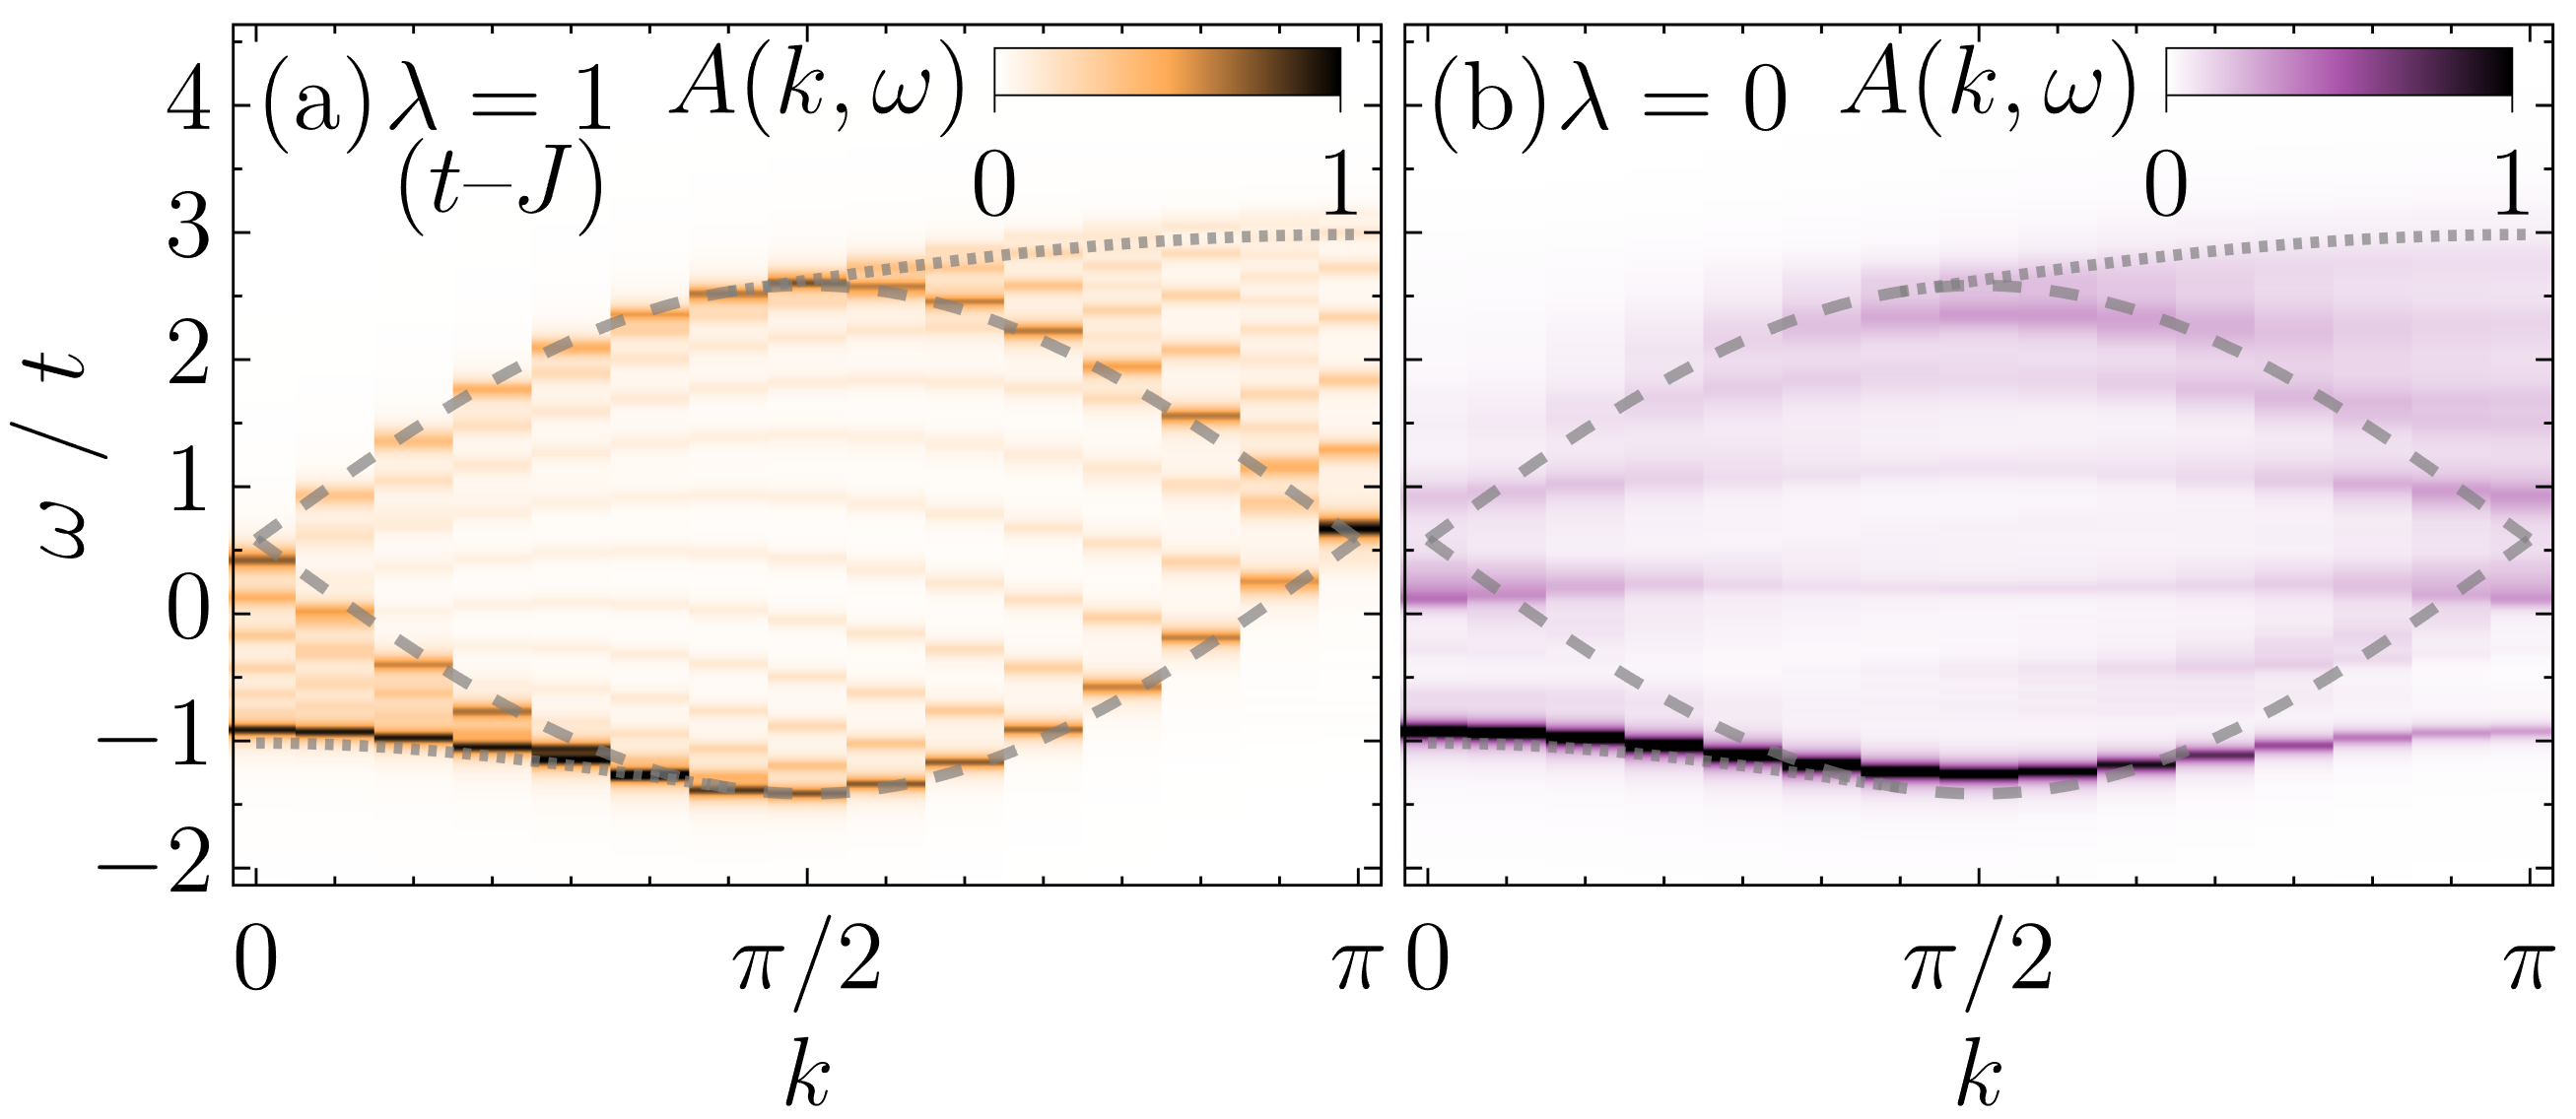
\includegraphics[width=\columnwidth]
    {fig_3.png}
\caption{
Properties of the excited state of the 1D $t$--$J$ model with a single hole
as probed by the spectral function $A(k,\omega)$: (a) with the magnon-magnon interactions correctly included
[$\lambda=1$ in \eqref{eq:model}];
(b) without the magnon-magnon interactions
[$\lambda=0$ in \eqref{eq:model}].
The dashed (dotted) lines in (a-b) show the holon (spinon) dispersion relations respectively, as obtained from the spin-charge separation Ansatz~\cite{Ede97, Kim97}. 
The highest intensity peak at lowest energy in (b) is the spin polaron quasiparticle peak.
Calculation performed on the \L~sites long periodic chain using exact diagonalization
and with $J=0.4t$.
}
\label{fig:spectra}
\end{figure}

{\it Interpretation \& critical magnon interactions}
A striking feature of the obtained results is that, at the qualitative level, the spin polaron solution to the single hole problem dictated by \eqref{eq:model} exists not only when the magnon-magnon attraction is switched off but also for all values of the magnon-magnon attraction except for the `critical' $\lambda = 1$,
which preserves the SU(2) symmetry
[the SU(2) symmetry is broken in the model once $\lambda \neq 1$ in \eqref{eq:model}, see \cite{SM}].
While this result can be verified using the observables used above, it is actually more instructive now to use a different observable [Fig.~\ref{fig:cn}(a-c)], for
it provides a more intuitive and simpler understanding of the results that follow. 


To this end we calculate the probability $c_n$ of finding a state with $n$ magnons forming a chain attached to one side of the single hole, in the ground state of \eqref{eq:model}, cf. Fig.~\ref{fig:cn}(c). The first result here is that only at the critical value of the magnon-magnon interactions $\lambda =1$ the $c_n$'s are the same for all $n$, 
consistent with spin-charge separation, cf. Fig.~\ref{fig:cn}(a). This is because, at $\lambda=1$ only, the cost of creating an extra magnon next to an existing magnon is precisely cancelled by their atraction. Hence, none of the magnons created by the mobile hole costs any energy apart from the first one, as long as they form a string. This, together with the magnon pair creation and annihilation terms [terms $\propto a_i a_j + h.c. $ in Eq.~(\ref{eq:model})], allows for constant $c_n$'s in the bulk of the chain.

Once $ \lambda \neq 1$ the probability $c_n$  is {\it never} a constant function of $n$ and spin-charge separation cannot take place [cf. Fig.~\ref{fig:cn}(a), {\it inter alia} note the distinct behavior for $\lambda =0.99$ and $\lambda =1 $]. This is due to the fact that for $\lambda \neq 1$ there can never be an exact `cancellation' between the magnon on-site and the interaction energy. In particular, for the physically interesting case of $0 \le \lambda <1$, that interpolates between the exact expression for the 1D $t$--$J$ model and the linear spin-wave approximation, $c_n$ decreases  superexponentially with increasing number of magnons $n$, cf.~Fig.~\ref{fig:cn}(a). This is due to the mobile hole exciting magnons whose energy cost grows linearly with their number. Hence, the total energy is optimised through a subtle competition between the hole polaronic energy and the magnon energy leading to the superexponentially suppressed probability of finding a configuration with an increasing number of magnons. This signals the onset of the string potential and the spin polaron picture,
just as e.g. in the 2D $t$--$J^z$ model~\cite{Bie19}.
  
\begin{figure}[t!]
    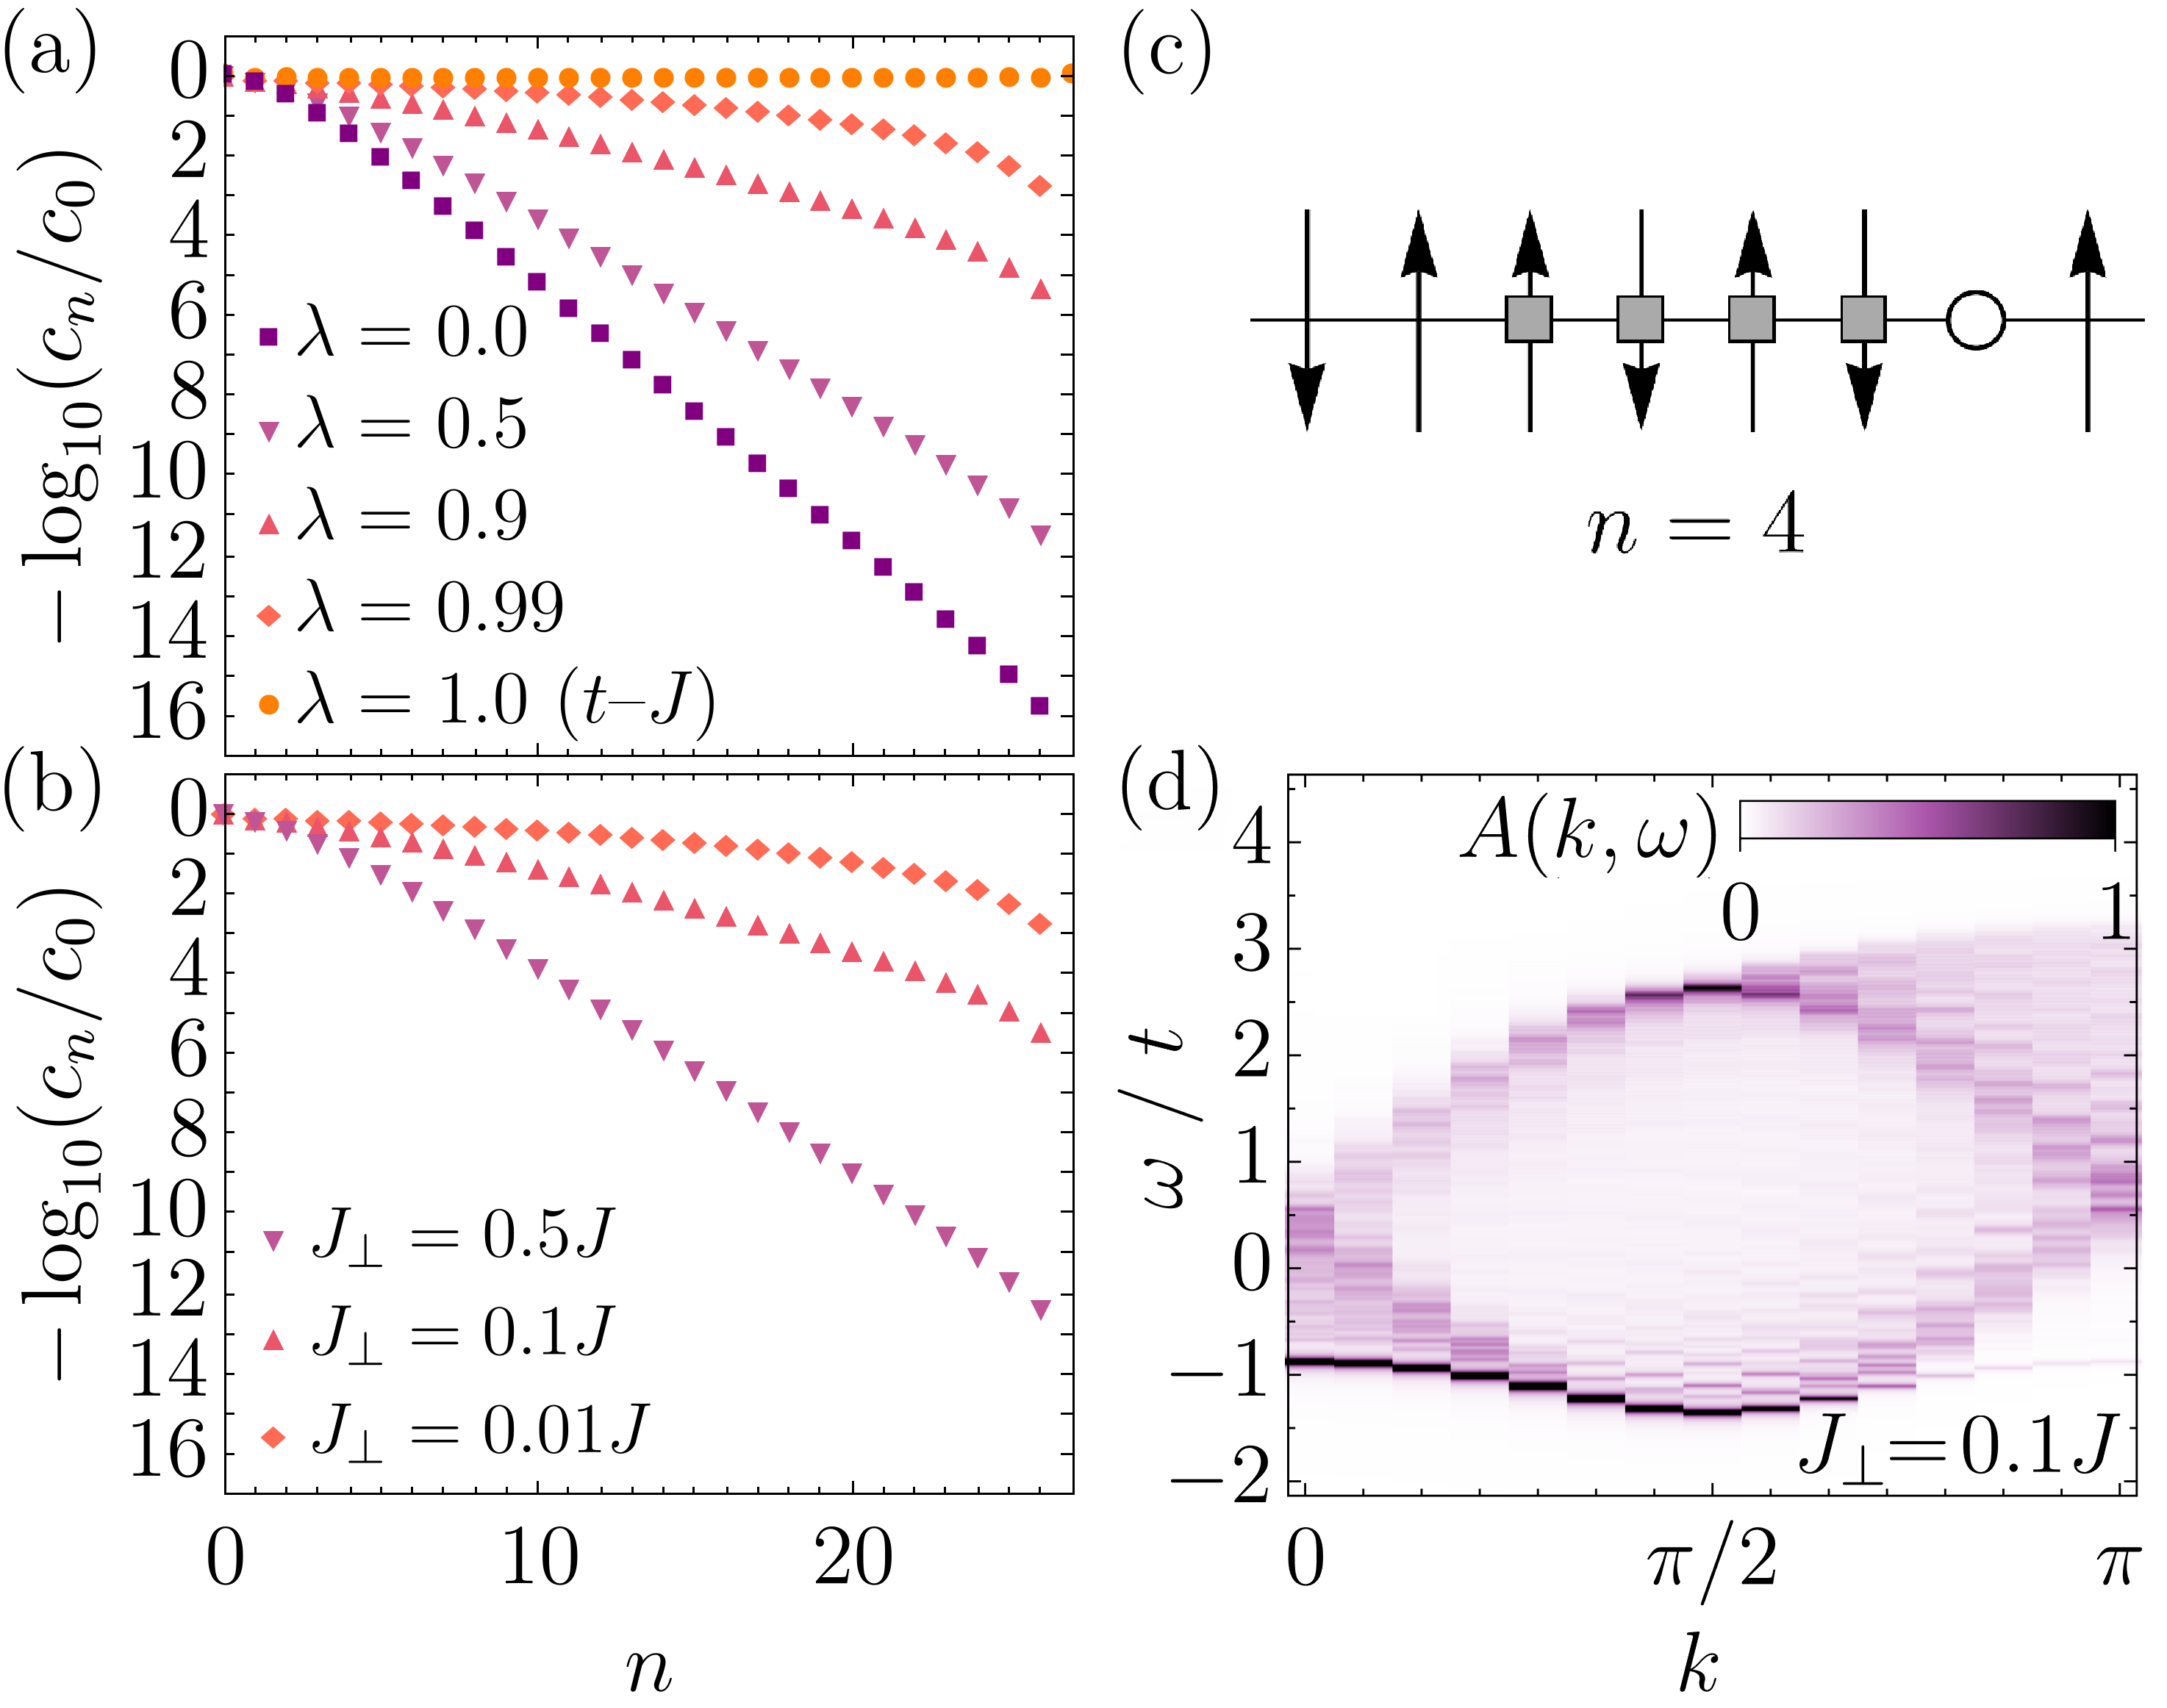
\includegraphics[width=\columnwidth]
    {fig_4.png}
\caption{
Properties of 1D $t$--$J$ model with a single hole and with: (a) {\it modified} strength of the magnon-magnon interactions [$\lambda$ in \eqref{eq:model}];
(b, d) {\it added} staggered magnetic field arising due to the coupling [$J_\perp / J$ 
in Eq. (1) in~\cite{SM}] to neighboring chains in a quasi-1D geometry, cf.~text and~\cite{SM}.
Panels (a-b) show probabilities $c_n$ of finding a configuration with $n$ consecutive magnons attached to one side of the hole in the ground state of the 
respective model; panel (c) shows a pictorial view of a configuration with $n=4$ magnons 
attached to the left side of the hole; panel (d) shows the spectral function $A(k,\omega)$ calculated for the 
1D $t$--$J$ model with added staggered magnetic field $J_\perp = 0.1J$.
All data obtained using exact diagonalization on the \L~sites periodic chain using $J=0.4t$.
}
\label{fig:cn}
\end{figure}


{\it Relevance for real materials} The existence of just one critical value of the magnon-magnon interactions [$\lambda =1$ in \eqref{eq:model}] stabilising the spin-charge separation solution leads to an important consequence for real materials. Due to the nature of atomic wavefunctions and crystal structures, the best-known `1D'
antiferromagnetic materials (cf. Sr$_2$CuO$_3$, SrCuO$_2$, or KCuF$_3$) are solely {\it quasi}-1D~\cite{Kojima1997, Matsuda1997, Lake2005}. A precise model of these materials should include a small but finite staggered magnetic field $J_\perp$ [see the Supplementary Material~\cite{SM} for details], which originates in the magnetic coupling between the spins on neighboring chains~\cite{Schulz1996, Essler1997, Sandvik1999}.
Importantly, the single-hole dynamics in a 1D $t$--$J$ model with staggered fields is qualitatively the same (and quantitatively very similar, as discussed in the Supplementary Material~\cite{SM}) as
that in a 1D $t$--$J$ model with magnon-magnon interactions (and XXZ anisotropy). Here, the strength of the staggered field can be mapped to the strength of the magnon-magnon interactions.
The reason for this is that the staggered field disrupts the above-discussed fine balance in the strict 1D $t$--$J$ model, between the on-site magnon energy and the magnon-magnon attraction. 
In this case, the mobile hole in the quasi-1D cuprates experiences the string potential and forms 
the spin polaron, cf.~Fig~\ref{fig:cn}(b). Therefore, the sensitivity to magnon interactions indicates that spin-charge separation is strictly speaking never realised in real materials.

One may wonder how to reconcile the above finding with the fact that ARPES experiments on quasi-1D materials have reported 
spin-charge separation~\cite{Kim96, Kim1997, Fujisawa1999, Koitzsch2006, Kim06}. That statement is based on the experimentally measured spectrum being similar 
to the one obtained for the 1D $t$--$J$ model, 
cf. Fig.~\ref{fig:spectra}(a) above \cite{Kim96, Kim1997, Fujisawa1999, Koitzsch2006, Kim06}. The salient fact is that the spectrum obtained for the 1D $t$--$J$
model with a realistic value of the staggered field $0<J_\perp \lesssim 0.1J$~\cite{SM}, cf.~Fig~\ref{fig:cn}(d), is {\it almost indistinguishable}
from the one of Fig.~\ref{fig:spectra}(a). 
In fact, for the available finite size calculations with the numerical broadening $\delta = 0.05 t$, 
the only visible difference between the two spectra lies in an extremely faint quasiparticle feature present for $k>\pi/2$. The latter
feature cannot be observed with the current ARPES resolution, especially at high temperature and with a typically
weaker signal for $k>\pi/2$ in ARPES. Thus, we conclude that ARPES on {\it quasi}-1D
cuprates is correctly-explained using the spin polaron picture, with its dominant cosine-like features interpreted
as the holon exciting a magnon at a vertex $\propto t |\cos k|$ (see above).


{\it Conclusions}
In this work we discussed the extent to which the concept of the spin polaron, well-known from the studies of a single hole in the 2D antiferromagnets~\cite{Shr88}, can be applied to the single hole problem in the 1D antiferromagnets. We find that {\it only} in the 1D SU(2) symmetric model the spin polaron is unstable to spin-charge separation due to the critical value of the magnon-magnon interactions. In contrast, the spin polaron quasiparticle is stable in the real {\it quasi}-1D antiferromagnets such as SrCuO$_2$, Sr$_2$CuO$_3$ or KCuF$_3$.
The surprising robustness of the spin polaron leaves us with a question whether this simple picture can be used to study also the higher-dimensional highly-doped antiferromagnets beyond the collapse of the long-range order.

\section*{Acknowledgements}
We thank Alberto Nocera and Steve Johnston for stimulating discussions.
We  kindly  acknowledge  support  by  the  (Polish)  National  Science  Centre  (NCN, Poland)  under  Projects  No. 2016/22/E/ST3/00560, 2016/23/B/ST3/00839, 2021/40/C/ST3/00177 as well as the Excellence Initiative of the University of Warsaw (`New Ideas' programme).
Y.W. acknowledge support from the National Science Foundation (NSF) award DMR-2132338.
M.B. acknowledges support from the Stewart Blusson Quantum Matter Institute and from NSERC. 
K.W. thanks the Stewart Blusson Quantum Matter Institute for the kind hospitality.
This research was carried out with the support of the Interdisciplinary Center for Mathematical and Computational Modeling at the University of Warsaw (ICM UW) under grant no G73-29.


For the purpose of Open Access, the authors have applied a CC-BY public copyright licence to any
Author Accepted Manuscript (AAM) version arising from this submission.
    

\begin{thebibliography}{59}%
    \makeatletter
    \providecommand \@ifxundefined [1]{%
     \@ifx{#1\undefined}
    }%
    \providecommand \@ifnum [1]{%
     \ifnum #1\expandafter \@firstoftwo
     \else \expandafter \@secondoftwo
     \fi
    }%
    \providecommand \@ifx [1]{%
     \ifx #1\expandafter \@firstoftwo
     \else \expandafter \@secondoftwo
     \fi
    }%
    \providecommand \natexlab [1]{#1}%
    \providecommand \enquote  [1]{``#1''}%
    \providecommand \bibnamefont  [1]{#1}%
    \providecommand \bibfnamefont [1]{#1}%
    \providecommand \citenamefont [1]{#1}%
    \providecommand \href@noop [0]{\@secondoftwo}%
    \providecommand \href [0]{\begingroup \@sanitize@url \@href}%
    \providecommand \@href[1]{\@@startlink{#1}\@@href}%
    \providecommand \@@href[1]{\endgroup#1\@@endlink}%
    \providecommand \@sanitize@url [0]{\catcode `\\12\catcode `\$12\catcode
      `\&12\catcode `\#12\catcode `\^12\catcode `\_12\catcode `\%12\relax}%
    \providecommand \@@startlink[1]{}%
    \providecommand \@@endlink[0]{}%
    \providecommand \url  [0]{\begingroup\@sanitize@url \@url }%
    \providecommand \@url [1]{\endgroup\@href {#1}{\urlprefix }}%
    \providecommand \urlprefix  [0]{URL }%
    \providecommand \Eprint [0]{\href }%
    \providecommand \doibase [0]{http://dx.doi.org/}%
    \providecommand \selectlanguage [0]{\@gobble}%
    \providecommand \bibinfo  [0]{\@secondoftwo}%
    \providecommand \bibfield  [0]{\@secondoftwo}%
    \providecommand \translation [1]{[#1]}%
    \providecommand \BibitemOpen [0]{}%
    \providecommand \bibitemStop [0]{}%
    \providecommand \bibitemNoStop [0]{.\EOS\space}%
    \providecommand \EOS [0]{\spacefactor3000\relax}%
    \providecommand \BibitemShut  [1]{\csname bibitem#1\endcsname}%
    \let\auto@bib@innerbib\@empty
    %</preamble>
    \bibitem [{\citenamefont {Khomskii}(2010)}]{Khomskii2010}%
      \BibitemOpen
      \bibfield  {author} {\bibinfo {author} {\bibfnamefont {D.~I.}\ \bibnamefont
      {Khomskii}},\ }\href@noop {} {\emph {\bibinfo {title} {Basic Aspects of the
      Quantum Theory of Solids: Order and Elementary Excitations}}}\ (\bibinfo
      {publisher} {Cambridge University Press},\ \bibinfo {address} {Cambridge},\
      \bibinfo {year} {2010})\BibitemShut {NoStop}%
    \bibitem [{\citenamefont {Zaanen}(2019)}]{Zaanen2019}%
      \BibitemOpen
      \bibfield  {author} {\bibinfo {author} {\bibfnamefont {J.}~\bibnamefont
      {Zaanen}},\ }\href {\doibase 10.21468/SciPostPhys.6.5.061} {\bibfield
      {journal} {\bibinfo  {journal} {SciPost Phys.}\ }\textbf {\bibinfo {volume}
      {6}},\ \bibinfo {pages} {61} (\bibinfo {year} {2019})}\BibitemShut {NoStop}%
    \bibitem [{\citenamefont {Kumar}\ \emph {et~al.}(2021)\citenamefont {Kumar},
      \citenamefont {Sachdev},\ and\ \citenamefont {Tripathi}}]{Kumar2021}%
      \BibitemOpen
      \bibfield  {author} {\bibinfo {author} {\bibfnamefont {A.}~\bibnamefont
      {Kumar}}, \bibinfo {author} {\bibfnamefont {S.}~\bibnamefont {Sachdev}}, \
      and\ \bibinfo {author} {\bibfnamefont {V.}~\bibnamefont {Tripathi}},\
      }\href@noop {} {\enquote {\bibinfo {title} {Quasiparticle metamorphosis in
      the random t-j model},}\ } (\bibinfo {year} {2021}),\ \Eprint
      {http://arxiv.org/abs/2112.01760} {arXiv:2112.01760 [cond-mat.str-el]}
      \BibitemShut {NoStop}%
    \bibitem [{\citenamefont {L\"auchli}\ and\ \citenamefont
      {Poilblanc}(2004)}]{Lauchli2004}%
      \BibitemOpen
      \bibfield  {author} {\bibinfo {author} {\bibfnamefont {A.}~\bibnamefont
      {L\"auchli}}\ and\ \bibinfo {author} {\bibfnamefont {D.}~\bibnamefont
      {Poilblanc}},\ }\href {\doibase 10.1103/PhysRevLett.92.236404} {\bibfield
      {journal} {\bibinfo  {journal} {Phys. Rev. Lett.}\ }\textbf {\bibinfo
      {volume} {92}},\ \bibinfo {pages} {236404} (\bibinfo {year}
      {2004})}\BibitemShut {NoStop}%
    \bibitem [{\citenamefont {Verresen}\ \emph {et~al.}(2019)\citenamefont
      {Verresen}, \citenamefont {Moessner},\ and\ \citenamefont
      {Pollmann}}]{Ver19}%
      \BibitemOpen
      \bibfield  {author} {\bibinfo {author} {\bibfnamefont {R.}~\bibnamefont
      {Verresen}}, \bibinfo {author} {\bibfnamefont {R.}~\bibnamefont {Moessner}},
      \ and\ \bibinfo {author} {\bibfnamefont {F.}~\bibnamefont {Pollmann}},\
      }\href {\doibase 10.1038/s41567-019-0535-3} {\bibfield  {journal} {\bibinfo
      {journal} {Nature Physics}\ }\textbf {\bibinfo {volume} {15}},\ \bibinfo
      {pages} {750} (\bibinfo {year} {2019})}\BibitemShut {NoStop}%
    \bibitem [{\citenamefont {Bulaevskii}\ \emph {et~al.}(1968)\citenamefont
      {Bulaevskii}, \citenamefont {Nagaev},\ and\ \citenamefont
      {Khomskii}}]{Bul68}%
      \BibitemOpen
      \bibfield  {author} {\bibinfo {author} {\bibfnamefont {L.~N.}\ \bibnamefont
      {Bulaevskii}}, \bibinfo {author} {\bibfnamefont {E.~L.}\ \bibnamefont
      {Nagaev}}, \ and\ \bibinfo {author} {\bibfnamefont {D.~I.}\ \bibnamefont
      {Khomskii}},\ }\href
      {http://www.jetp.ac.ru/cgi-bin/e/index/e/27/5/p836?a=list} {\bibfield
      {journal} {\bibinfo  {journal} {JETP}\ }\textbf {\bibinfo {volume} {27}},\
      \bibinfo {pages} {836} (\bibinfo {year} {1968})}\BibitemShut {NoStop}%
    \bibitem [{\citenamefont {Schmitt-Rink}\ \emph {et~al.}(1988)\citenamefont
      {Schmitt-Rink}, \citenamefont {Varma},\ and\ \citenamefont
      {Ruckenstein}}]{Sch88}%
      \BibitemOpen
      \bibfield  {author} {\bibinfo {author} {\bibfnamefont {S.}~\bibnamefont
      {Schmitt-Rink}}, \bibinfo {author} {\bibfnamefont {C.~M.}\ \bibnamefont
      {Varma}}, \ and\ \bibinfo {author} {\bibfnamefont {A.~E.}\ \bibnamefont
      {Ruckenstein}},\ }\href {\doibase 10.1103/PhysRevLett.60.2793} {\bibfield
      {journal} {\bibinfo  {journal} {Phys. Rev. Lett.}\ }\textbf {\bibinfo
      {volume} {60}},\ \bibinfo {pages} {2793} (\bibinfo {year}
      {1988})}\BibitemShut {NoStop}%
    \bibitem [{\citenamefont {Mart\'inez}\ and\ \citenamefont
      {Horsch}(1991)}]{Mar91}%
      \BibitemOpen
      \bibfield  {author} {\bibinfo {author} {\bibfnamefont {G.}~\bibnamefont
      {Mart\'inez}}\ and\ \bibinfo {author} {\bibfnamefont {P.}~\bibnamefont
      {Horsch}},\ }\href {\doibase 10.1103/PhysRevB.44.317} {\bibfield  {journal}
      {\bibinfo  {journal} {Phys. Rev. B}\ }\textbf {\bibinfo {volume} {44}},\
      \bibinfo {pages} {317} (\bibinfo {year} {1991})}\BibitemShut {NoStop}%
    \bibitem [{\citenamefont {Grusdt}\ \emph {et~al.}(2018)\citenamefont {Grusdt},
      \citenamefont {K\'anasz-Nagy}, \citenamefont {Bohrdt}, \citenamefont {Chiu},
      \citenamefont {Ji}, \citenamefont {Greiner}, \citenamefont {Greif},\ and\
      \citenamefont {Demler}}]{Gru18}%
      \BibitemOpen
      \bibfield  {author} {\bibinfo {author} {\bibfnamefont {F.}~\bibnamefont
      {Grusdt}}, \bibinfo {author} {\bibfnamefont {M.}~\bibnamefont
      {K\'anasz-Nagy}}, \bibinfo {author} {\bibfnamefont {A.}~\bibnamefont
      {Bohrdt}}, \bibinfo {author} {\bibfnamefont {C.~S.}\ \bibnamefont {Chiu}},
      \bibinfo {author} {\bibfnamefont {G.}~\bibnamefont {Ji}}, \bibinfo {author}
      {\bibfnamefont {M.}~\bibnamefont {Greiner}}, \bibinfo {author} {\bibfnamefont
      {D.}~\bibnamefont {Greif}}, \ and\ \bibinfo {author} {\bibfnamefont
      {E.}~\bibnamefont {Demler}},\ }\href {\doibase 10.1103/PhysRevX.8.011046}
      {\bibfield  {journal} {\bibinfo  {journal} {Phys. Rev. X}\ }\textbf {\bibinfo
      {volume} {8}},\ \bibinfo {pages} {011046} (\bibinfo {year}
      {2018})}\BibitemShut {NoStop}%
    \bibitem [{\citenamefont {{Chiu}}\ \emph {et~al.}(2019)\citenamefont {{Chiu}},
      \citenamefont {{Ji}}, \citenamefont {{Bohrdt}}, \citenamefont {{Xu}},
      \citenamefont {{Knap}}, \citenamefont {{Demler}}, \citenamefont {{Grusdt}},
      \citenamefont {{Greiner}},\ and\ \citenamefont {{Greif}}}]{Chi18}%
      \BibitemOpen
      \bibfield  {author} {\bibinfo {author} {\bibfnamefont {C.~S.}\ \bibnamefont
      {{Chiu}}}, \bibinfo {author} {\bibfnamefont {G.}~\bibnamefont {{Ji}}},
      \bibinfo {author} {\bibfnamefont {A.}~\bibnamefont {{Bohrdt}}}, \bibinfo
      {author} {\bibfnamefont {M.}~\bibnamefont {{Xu}}}, \bibinfo {author}
      {\bibfnamefont {M.}~\bibnamefont {{Knap}}}, \bibinfo {author} {\bibfnamefont
      {E.}~\bibnamefont {{Demler}}}, \bibinfo {author} {\bibfnamefont
      {F.}~\bibnamefont {{Grusdt}}}, \bibinfo {author} {\bibfnamefont
      {M.}~\bibnamefont {{Greiner}}}, \ and\ \bibinfo {author} {\bibfnamefont
      {D.}~\bibnamefont {{Greif}}},\ }\href {\doibase 10.1126/science.aav3587}
      {\bibfield  {journal} {\bibinfo  {journal} {Science}\ }\textbf {\bibinfo
      {volume} {365}},\ \bibinfo {pages} {251} (\bibinfo {year}
      {2019})}\BibitemShut {NoStop}%
    \bibitem [{\citenamefont {Koepsell}\ \emph {et~al.}(2019)\citenamefont
      {Koepsell}, \citenamefont {Vijayan}, \citenamefont {Sompet}, \citenamefont
      {Grusdt}, \citenamefont {Hilker}, \citenamefont {Demler}, \citenamefont
      {Salomon}, \citenamefont {Bloch},\ and\ \citenamefont
      {Gross}}]{Koepsell2019}%
      \BibitemOpen
      \bibfield  {author} {\bibinfo {author} {\bibfnamefont {J.}~\bibnamefont
      {Koepsell}}, \bibinfo {author} {\bibfnamefont {J.}~\bibnamefont {Vijayan}},
      \bibinfo {author} {\bibfnamefont {P.}~\bibnamefont {Sompet}}, \bibinfo
      {author} {\bibfnamefont {F.}~\bibnamefont {Grusdt}}, \bibinfo {author}
      {\bibfnamefont {T.~A.}\ \bibnamefont {Hilker}}, \bibinfo {author}
      {\bibfnamefont {E.}~\bibnamefont {Demler}}, \bibinfo {author} {\bibfnamefont
      {G.}~\bibnamefont {Salomon}}, \bibinfo {author} {\bibfnamefont
      {I.}~\bibnamefont {Bloch}}, \ and\ \bibinfo {author} {\bibfnamefont
      {C.}~\bibnamefont {Gross}},\ }\href {\doibase 10.1038/s41586-019-1463-1}
      {\bibfield  {journal} {\bibinfo  {journal} {Nature}\ }\textbf {\bibinfo
      {volume} {572}},\ \bibinfo {pages} {358} (\bibinfo {year}
      {2019})}\BibitemShut {NoStop}%
    \bibitem [{\citenamefont {Koepsell}\ \emph {et~al.}(2021)\citenamefont
      {Koepsell}, \citenamefont {Bourgund}, \citenamefont {Sompet}, \citenamefont
      {Hirthe}, \citenamefont {Bohrdt}, \citenamefont {Wang}, \citenamefont
      {Grusdt}, \citenamefont {Demler}, \citenamefont {Salomon}, \citenamefont
      {Gross},\ and\ \citenamefont {Bloch}}]{Koepsell2021}%
      \BibitemOpen
      \bibfield  {author} {\bibinfo {author} {\bibfnamefont {J.}~\bibnamefont
      {Koepsell}}, \bibinfo {author} {\bibfnamefont {D.}~\bibnamefont {Bourgund}},
      \bibinfo {author} {\bibfnamefont {P.}~\bibnamefont {Sompet}}, \bibinfo
      {author} {\bibfnamefont {S.}~\bibnamefont {Hirthe}}, \bibinfo {author}
      {\bibfnamefont {A.}~\bibnamefont {Bohrdt}}, \bibinfo {author} {\bibfnamefont
      {Y.}~\bibnamefont {Wang}}, \bibinfo {author} {\bibfnamefont {F.}~\bibnamefont
      {Grusdt}}, \bibinfo {author} {\bibfnamefont {E.}~\bibnamefont {Demler}},
      \bibinfo {author} {\bibfnamefont {G.}~\bibnamefont {Salomon}}, \bibinfo
      {author} {\bibfnamefont {C.}~\bibnamefont {Gross}}, \ and\ \bibinfo {author}
      {\bibfnamefont {I.}~\bibnamefont {Bloch}},\ }\href {\doibase
      10.1126/science.abe7165} {\bibfield  {journal} {\bibinfo  {journal}
      {Science}\ }\textbf {\bibinfo {volume} {374}},\ \bibinfo {pages} {82}
      (\bibinfo {year} {2021})}\BibitemShut {NoStop}%
    \bibitem [{\citenamefont {Wang}\ \emph {et~al.}(2021)\citenamefont {Wang},
      \citenamefont {Bohrdt}, \citenamefont {Ding}, \citenamefont {Koepsell},
      \citenamefont {Demler},\ and\ \citenamefont {Grusdt}}]{Wang2021}%
      \BibitemOpen
      \bibfield  {author} {\bibinfo {author} {\bibfnamefont {Y.}~\bibnamefont
      {Wang}}, \bibinfo {author} {\bibfnamefont {A.}~\bibnamefont {Bohrdt}},
      \bibinfo {author} {\bibfnamefont {S.}~\bibnamefont {Ding}}, \bibinfo {author}
      {\bibfnamefont {J.}~\bibnamefont {Koepsell}}, \bibinfo {author}
      {\bibfnamefont {E.}~\bibnamefont {Demler}}, \ and\ \bibinfo {author}
      {\bibfnamefont {F.}~\bibnamefont {Grusdt}},\ }\href {\doibase
      10.1103/PhysRevResearch.3.033204} {\bibfield  {journal} {\bibinfo  {journal}
      {Phys. Rev. Research}\ }\textbf {\bibinfo {volume} {3}},\ \bibinfo {pages}
      {033204} (\bibinfo {year} {2021})}\BibitemShut {NoStop}%
    \bibitem [{\citenamefont {Bohrdt}\ \emph
      {et~al.}(2021{\natexlab{a}})\citenamefont {Bohrdt}, \citenamefont {Wang},
      \citenamefont {Koepsell}, \citenamefont {K\'anasz-Nagy}, \citenamefont
      {Demler},\ and\ \citenamefont {Grusdt}}]{Bohrdt2021_01}%
      \BibitemOpen
      \bibfield  {author} {\bibinfo {author} {\bibfnamefont {A.}~\bibnamefont
      {Bohrdt}}, \bibinfo {author} {\bibfnamefont {Y.}~\bibnamefont {Wang}},
      \bibinfo {author} {\bibfnamefont {J.}~\bibnamefont {Koepsell}}, \bibinfo
      {author} {\bibfnamefont {M.}~\bibnamefont {K\'anasz-Nagy}}, \bibinfo {author}
      {\bibfnamefont {E.}~\bibnamefont {Demler}}, \ and\ \bibinfo {author}
      {\bibfnamefont {F.}~\bibnamefont {Grusdt}},\ }\href {\doibase
      10.1103/PhysRevLett.126.026401} {\bibfield  {journal} {\bibinfo  {journal}
      {Phys. Rev. Lett.}\ }\textbf {\bibinfo {volume} {126}},\ \bibinfo {pages}
      {026401} (\bibinfo {year} {2021}{\natexlab{a}})}\BibitemShut {NoStop}%
    \bibitem [{\citenamefont {Lieb}\ and\ \citenamefont {Wu}(1968)}]{Lieb1968}%
      \BibitemOpen
      \bibfield  {author} {\bibinfo {author} {\bibfnamefont {E.~H.}\ \bibnamefont
      {Lieb}}\ and\ \bibinfo {author} {\bibfnamefont {F.~Y.}\ \bibnamefont {Wu}},\
      }\href {\doibase 10.1103/physrevlett.20.1445} {\bibfield  {journal} {\bibinfo
       {journal} {Physical Review Letters}\ }\textbf {\bibinfo {volume} {20}},\
      \bibinfo {pages} {1445} (\bibinfo {year} {1968})}\BibitemShut {NoStop}%
    \bibitem [{\citenamefont {Voit}(1995)}]{Voi95}%
      \BibitemOpen
      \bibfield  {author} {\bibinfo {author} {\bibfnamefont {J.}~\bibnamefont
      {Voit}},\ }\href {http://stacks.iop.org/0034-4885/58/i=9/a=002} {\bibfield
      {journal} {\bibinfo  {journal} {Reports on Progress in Physics}\ }\textbf
      {\bibinfo {volume} {58}},\ \bibinfo {pages} {977} (\bibinfo {year}
      {1995})}\BibitemShut {NoStop}%
    \bibitem [{\citenamefont {Kim}\ \emph {et~al.}(1996)\citenamefont {Kim},
      \citenamefont {Matsuura}, \citenamefont {Shen}, \citenamefont {Motoyama},
      \citenamefont {Eisaki}, \citenamefont {Uchida}, \citenamefont {Tohyama},\
      and\ \citenamefont {Maekawa}}]{Kim96}%
      \BibitemOpen
      \bibfield  {author} {\bibinfo {author} {\bibfnamefont {C.}~\bibnamefont
      {Kim}}, \bibinfo {author} {\bibfnamefont {A.~Y.}\ \bibnamefont {Matsuura}},
      \bibinfo {author} {\bibfnamefont {Z.-X.}\ \bibnamefont {Shen}}, \bibinfo
      {author} {\bibfnamefont {N.}~\bibnamefont {Motoyama}}, \bibinfo {author}
      {\bibfnamefont {H.}~\bibnamefont {Eisaki}}, \bibinfo {author} {\bibfnamefont
      {S.}~\bibnamefont {Uchida}}, \bibinfo {author} {\bibfnamefont
      {T.}~\bibnamefont {Tohyama}}, \ and\ \bibinfo {author} {\bibfnamefont
      {S.}~\bibnamefont {Maekawa}},\ }\href {\doibase 10.1103/PhysRevLett.77.4054}
      {\bibfield  {journal} {\bibinfo  {journal} {Phys. Rev. Lett.}\ }\textbf
      {\bibinfo {volume} {77}},\ \bibinfo {pages} {4054} (\bibinfo {year}
      {1996})}\BibitemShut {NoStop}%
    \bibitem [{\citenamefont {Kim}\ \emph {et~al.}(1997{\natexlab{a}})\citenamefont
      {Kim}, \citenamefont {Shen}, \citenamefont {Motoyama}, \citenamefont
      {Eisaki}, \citenamefont {Uchida}, \citenamefont {Tohyama},\ and\
      \citenamefont {Maekawa}}]{Kim1997}%
      \BibitemOpen
      \bibfield  {author} {\bibinfo {author} {\bibfnamefont {C.}~\bibnamefont
      {Kim}}, \bibinfo {author} {\bibfnamefont {Z.-X.}\ \bibnamefont {Shen}},
      \bibinfo {author} {\bibfnamefont {N.}~\bibnamefont {Motoyama}}, \bibinfo
      {author} {\bibfnamefont {H.}~\bibnamefont {Eisaki}}, \bibinfo {author}
      {\bibfnamefont {S.}~\bibnamefont {Uchida}}, \bibinfo {author} {\bibfnamefont
      {T.}~\bibnamefont {Tohyama}}, \ and\ \bibinfo {author} {\bibfnamefont
      {S.}~\bibnamefont {Maekawa}},\ }\href {\doibase 10.1103/PhysRevB.56.15589}
      {\bibfield  {journal} {\bibinfo  {journal} {Phys. Rev. B}\ }\textbf {\bibinfo
      {volume} {56}},\ \bibinfo {pages} {15589} (\bibinfo {year}
      {1997}{\natexlab{a}})}\BibitemShut {NoStop}%
    \bibitem [{\citenamefont {Fujisawa}\ \emph {et~al.}(1999)\citenamefont
      {Fujisawa}, \citenamefont {Yokoya}, \citenamefont {Takahashi}, \citenamefont
      {Miyasaka}, \citenamefont {Kibune},\ and\ \citenamefont
      {Takagi}}]{Fujisawa1999}%
      \BibitemOpen
      \bibfield  {author} {\bibinfo {author} {\bibfnamefont {H.}~\bibnamefont
      {Fujisawa}}, \bibinfo {author} {\bibfnamefont {T.}~\bibnamefont {Yokoya}},
      \bibinfo {author} {\bibfnamefont {T.}~\bibnamefont {Takahashi}}, \bibinfo
      {author} {\bibfnamefont {S.}~\bibnamefont {Miyasaka}}, \bibinfo {author}
      {\bibfnamefont {M.}~\bibnamefont {Kibune}}, \ and\ \bibinfo {author}
      {\bibfnamefont {H.}~\bibnamefont {Takagi}},\ }\href {\doibase
      10.1103/PhysRevB.59.7358} {\bibfield  {journal} {\bibinfo  {journal} {Phys.
      Rev. B}\ }\textbf {\bibinfo {volume} {59}},\ \bibinfo {pages} {7358}
      (\bibinfo {year} {1999})}\BibitemShut {NoStop}%
    \bibitem [{\citenamefont {Poilblanc}\ \emph {et~al.}(2006)\citenamefont
      {Poilblanc}, \citenamefont {L\"auchli}, \citenamefont {Mambrini},\ and\
      \citenamefont {Mila}}]{Poilblanc2006}%
      \BibitemOpen
      \bibfield  {author} {\bibinfo {author} {\bibfnamefont {D.}~\bibnamefont
      {Poilblanc}}, \bibinfo {author} {\bibfnamefont {A.}~\bibnamefont
      {L\"auchli}}, \bibinfo {author} {\bibfnamefont {M.}~\bibnamefont {Mambrini}},
      \ and\ \bibinfo {author} {\bibfnamefont {F.}~\bibnamefont {Mila}},\ }\href
      {\doibase 10.1103/PhysRevB.73.100403} {\bibfield  {journal} {\bibinfo
      {journal} {Phys. Rev. B}\ }\textbf {\bibinfo {volume} {73}},\ \bibinfo
      {pages} {100403} (\bibinfo {year} {2006})}\BibitemShut {NoStop}%
    \bibitem [{\citenamefont {Koitzsch}\ \emph {et~al.}(2006)\citenamefont
      {Koitzsch}, \citenamefont {Borisenko}, \citenamefont {Geck}, \citenamefont
      {Zabolotnyy}, \citenamefont {Knupfer}, \citenamefont {Fink}, \citenamefont
      {Ribeiro}, \citenamefont {B\"uchner},\ and\ \citenamefont
      {Follath}}]{Koitzsch2006}%
      \BibitemOpen
      \bibfield  {author} {\bibinfo {author} {\bibfnamefont {A.}~\bibnamefont
      {Koitzsch}}, \bibinfo {author} {\bibfnamefont {S.~V.}\ \bibnamefont
      {Borisenko}}, \bibinfo {author} {\bibfnamefont {J.}~\bibnamefont {Geck}},
      \bibinfo {author} {\bibfnamefont {V.~B.}\ \bibnamefont {Zabolotnyy}},
      \bibinfo {author} {\bibfnamefont {M.}~\bibnamefont {Knupfer}}, \bibinfo
      {author} {\bibfnamefont {J.}~\bibnamefont {Fink}}, \bibinfo {author}
      {\bibfnamefont {P.}~\bibnamefont {Ribeiro}}, \bibinfo {author} {\bibfnamefont
      {B.}~\bibnamefont {B\"uchner}}, \ and\ \bibinfo {author} {\bibfnamefont
      {R.}~\bibnamefont {Follath}},\ }\href {\doibase 10.1103/PhysRevB.73.201101}
      {\bibfield  {journal} {\bibinfo  {journal} {Phys. Rev. B}\ }\textbf {\bibinfo
      {volume} {73}},\ \bibinfo {pages} {201101} (\bibinfo {year}
      {2006})}\BibitemShut {NoStop}%
    \bibitem [{\citenamefont {Kim}\ \emph {et~al.}(2006)\citenamefont {Kim},
      \citenamefont {Koh}, \citenamefont {Rotenberg}, \citenamefont {Oh},
      \citenamefont {Eisaki}, \citenamefont {Motoyama}, \citenamefont {Uchida},
      \citenamefont {Tohyama}, \citenamefont {Maekawa}, \citenamefont {Shen},\ and\
      \citenamefont {Kim}}]{Kim06}%
      \BibitemOpen
      \bibfield  {author} {\bibinfo {author} {\bibfnamefont {B.~J.}\ \bibnamefont
      {Kim}}, \bibinfo {author} {\bibfnamefont {H.}~\bibnamefont {Koh}}, \bibinfo
      {author} {\bibfnamefont {E.}~\bibnamefont {Rotenberg}}, \bibinfo {author}
      {\bibfnamefont {S.-J.}\ \bibnamefont {Oh}}, \bibinfo {author} {\bibfnamefont
      {H.}~\bibnamefont {Eisaki}}, \bibinfo {author} {\bibfnamefont
      {N.}~\bibnamefont {Motoyama}}, \bibinfo {author} {\bibfnamefont
      {S.}~\bibnamefont {Uchida}}, \bibinfo {author} {\bibfnamefont
      {T.}~\bibnamefont {Tohyama}}, \bibinfo {author} {\bibfnamefont
      {S.}~\bibnamefont {Maekawa}}, \bibinfo {author} {\bibfnamefont {Z.-X.}\
      \bibnamefont {Shen}}, \ and\ \bibinfo {author} {\bibfnamefont
      {C.}~\bibnamefont {Kim}},\ }\href {\doibase 10.1038/nphys316} {\bibfield
      {journal} {\bibinfo  {journal} {Nature Physics}\ }\textbf {\bibinfo {volume}
      {2}},\ \bibinfo {pages} {397} (\bibinfo {year} {2006})}\BibitemShut {NoStop}%
    \bibitem [{\citenamefont {Vijayan}\ \emph {et~al.}(2020)\citenamefont
      {Vijayan}, \citenamefont {Sompet}, \citenamefont {Salomon}, \citenamefont
      {Koepsell}, \citenamefont {Hirthe}, \citenamefont {Bohrdt}, \citenamefont
      {Grusdt}, \citenamefont {Bloch},\ and\ \citenamefont {Gross}}]{Jayadev2020}%
      \BibitemOpen
      \bibfield  {author} {\bibinfo {author} {\bibfnamefont {J.}~\bibnamefont
      {Vijayan}}, \bibinfo {author} {\bibfnamefont {P.}~\bibnamefont {Sompet}},
      \bibinfo {author} {\bibfnamefont {G.}~\bibnamefont {Salomon}}, \bibinfo
      {author} {\bibfnamefont {J.}~\bibnamefont {Koepsell}}, \bibinfo {author}
      {\bibfnamefont {S.}~\bibnamefont {Hirthe}}, \bibinfo {author} {\bibfnamefont
      {A.}~\bibnamefont {Bohrdt}}, \bibinfo {author} {\bibfnamefont
      {F.}~\bibnamefont {Grusdt}}, \bibinfo {author} {\bibfnamefont
      {I.}~\bibnamefont {Bloch}}, \ and\ \bibinfo {author} {\bibfnamefont
      {C.}~\bibnamefont {Gross}},\ }\href {\doibase 10.1126/science.aay2354}
      {\bibfield  {journal} {\bibinfo  {journal} {Science}\ }\textbf {\bibinfo
      {volume} {367}},\ \bibinfo {pages} {186} (\bibinfo {year}
      {2020})}\BibitemShut {NoStop}%
    \bibitem [{\citenamefont {Giamarchi}(2003)}]{Giamarchi2003}%
      \BibitemOpen
      \bibfield  {author} {\bibinfo {author} {\bibfnamefont {T.}~\bibnamefont
      {Giamarchi}},\ }\href {\doibase 10.1093/acprof:oso/9780198525004.001.0001}
      {\emph {\bibinfo {title} {Quantum Physics in One Dimension}}}\ (\bibinfo
      {publisher} {Oxford University Press},\ \bibinfo {year} {2003})\BibitemShut
      {NoStop}%
    \bibitem [{Note1()}]{Note1}%
      \BibitemOpen
      \bibinfo {note} {Interestingly, this situation is distinct from the one
      reported in~\cite {Ver19}, in which interactions {\protect \it support} the
      stability of a quasiparticle.}\BibitemShut {Stop}%
    \bibitem [{\citenamefont {Kojima}\ \emph {et~al.}(1997)\citenamefont {Kojima},
      \citenamefont {Fudamoto}, \citenamefont {Larkin}, \citenamefont {Luke},
      \citenamefont {Merrin}, \citenamefont {Nachumi}, \citenamefont {Uemura},
      \citenamefont {Motoyama}, \citenamefont {Eisaki}, \citenamefont {Uchida},
      \citenamefont {Yamada}, \citenamefont {Endoh}, \citenamefont {Hosoya},
      \citenamefont {Sternlieb},\ and\ \citenamefont {Shirane}}]{Kojima1997}%
      \BibitemOpen
      \bibfield  {author} {\bibinfo {author} {\bibfnamefont {K.~M.}\ \bibnamefont
      {Kojima}}, \bibinfo {author} {\bibfnamefont {Y.}~\bibnamefont {Fudamoto}},
      \bibinfo {author} {\bibfnamefont {M.}~\bibnamefont {Larkin}}, \bibinfo
      {author} {\bibfnamefont {G.~M.}\ \bibnamefont {Luke}}, \bibinfo {author}
      {\bibfnamefont {J.}~\bibnamefont {Merrin}}, \bibinfo {author} {\bibfnamefont
      {B.}~\bibnamefont {Nachumi}}, \bibinfo {author} {\bibfnamefont {Y.~J.}\
      \bibnamefont {Uemura}}, \bibinfo {author} {\bibfnamefont {N.}~\bibnamefont
      {Motoyama}}, \bibinfo {author} {\bibfnamefont {H.}~\bibnamefont {Eisaki}},
      \bibinfo {author} {\bibfnamefont {S.}~\bibnamefont {Uchida}}, \bibinfo
      {author} {\bibfnamefont {K.}~\bibnamefont {Yamada}}, \bibinfo {author}
      {\bibfnamefont {Y.}~\bibnamefont {Endoh}}, \bibinfo {author} {\bibfnamefont
      {S.}~\bibnamefont {Hosoya}}, \bibinfo {author} {\bibfnamefont {B.~J.}\
      \bibnamefont {Sternlieb}}, \ and\ \bibinfo {author} {\bibfnamefont
      {G.}~\bibnamefont {Shirane}},\ }\href {\doibase 10.1103/PhysRevLett.78.1787}
      {\bibfield  {journal} {\bibinfo  {journal} {Phys. Rev. Lett.}\ }\textbf
      {\bibinfo {volume} {78}},\ \bibinfo {pages} {1787} (\bibinfo {year}
      {1997})}\BibitemShut {NoStop}%
    \bibitem [{\citenamefont {Matsuda}\ \emph {et~al.}(1997)\citenamefont
      {Matsuda}, \citenamefont {Katsumata}, \citenamefont {Kojima}, \citenamefont
      {Larkin}, \citenamefont {Luke}, \citenamefont {Merrin}, \citenamefont
      {Nachumi}, \citenamefont {Uemura}, \citenamefont {Eisaki}, \citenamefont
      {Motoyama}, \citenamefont {Uchida},\ and\ \citenamefont
      {Shirane}}]{Matsuda1997}%
      \BibitemOpen
      \bibfield  {author} {\bibinfo {author} {\bibfnamefont {M.}~\bibnamefont
      {Matsuda}}, \bibinfo {author} {\bibfnamefont {K.}~\bibnamefont {Katsumata}},
      \bibinfo {author} {\bibfnamefont {K.~M.}\ \bibnamefont {Kojima}}, \bibinfo
      {author} {\bibfnamefont {M.}~\bibnamefont {Larkin}}, \bibinfo {author}
      {\bibfnamefont {G.~M.}\ \bibnamefont {Luke}}, \bibinfo {author}
      {\bibfnamefont {J.}~\bibnamefont {Merrin}}, \bibinfo {author} {\bibfnamefont
      {B.}~\bibnamefont {Nachumi}}, \bibinfo {author} {\bibfnamefont {Y.~J.}\
      \bibnamefont {Uemura}}, \bibinfo {author} {\bibfnamefont {H.}~\bibnamefont
      {Eisaki}}, \bibinfo {author} {\bibfnamefont {N.}~\bibnamefont {Motoyama}},
      \bibinfo {author} {\bibfnamefont {S.}~\bibnamefont {Uchida}}, \ and\ \bibinfo
      {author} {\bibfnamefont {G.}~\bibnamefont {Shirane}},\ }\href {\doibase
      10.1103/PhysRevB.55.R11953} {\bibfield  {journal} {\bibinfo  {journal} {Phys.
      Rev. B}\ }\textbf {\bibinfo {volume} {55}},\ \bibinfo {pages} {R11953}
      (\bibinfo {year} {1997})}\BibitemShut {NoStop}%
    \bibitem [{\citenamefont {Lake}\ \emph {et~al.}(2005)\citenamefont {Lake},
      \citenamefont {Tennant}, \citenamefont {Frost},\ and\ \citenamefont
      {Nagler}}]{Lake2005}%
      \BibitemOpen
      \bibfield  {author} {\bibinfo {author} {\bibfnamefont {B.}~\bibnamefont
      {Lake}}, \bibinfo {author} {\bibfnamefont {D.~A.}\ \bibnamefont {Tennant}},
      \bibinfo {author} {\bibfnamefont {C.~D.}\ \bibnamefont {Frost}}, \ and\
      \bibinfo {author} {\bibfnamefont {S.~E.}\ \bibnamefont {Nagler}},\ }\href
      {\doibase 10.1038/nmat1327} {\bibfield  {journal} {\bibinfo  {journal}
      {Nature Materials}\ }\textbf {\bibinfo {volume} {4}},\ \bibinfo {pages} {329}
      (\bibinfo {year} {2005})}\BibitemShut {NoStop}%
    \bibitem [{\citenamefont {Sobota}\ \emph {et~al.}(2021)\citenamefont {Sobota},
      \citenamefont {He},\ and\ \citenamefont {Shen}}]{Sobota2021}%
      \BibitemOpen
      \bibfield  {author} {\bibinfo {author} {\bibfnamefont {J.~A.}\ \bibnamefont
      {Sobota}}, \bibinfo {author} {\bibfnamefont {Y.}~\bibnamefont {He}}, \ and\
      \bibinfo {author} {\bibfnamefont {Z.-X.}\ \bibnamefont {Shen}},\ }\href
      {\doibase 10.1103/RevModPhys.93.025006} {\bibfield  {journal} {\bibinfo
      {journal} {Rev. Mod. Phys.}\ }\textbf {\bibinfo {volume} {93}},\ \bibinfo
      {pages} {025006} (\bibinfo {year} {2021})}\BibitemShut {NoStop}%
    \bibitem [{\citenamefont {Bon\ifmmode~\check{c}\else \v{c}\fi{}a}\ and\
      \citenamefont {Prelov\ifmmode~\check{s}\else
      \v{s}\fi{}ek}(1992)}]{Bonca1992}%
      \BibitemOpen
      \bibfield  {author} {\bibinfo {author} {\bibfnamefont {J.}~\bibnamefont
      {Bon\ifmmode~\check{c}\else \v{c}\fi{}a}}\ and\ \bibinfo {author}
      {\bibfnamefont {P.}~\bibnamefont {Prelov\ifmmode~\check{s}\else
      \v{s}\fi{}ek}},\ }\href {\doibase 10.1103/PhysRevB.46.5705} {\bibfield
      {journal} {\bibinfo  {journal} {Phys. Rev. B}\ }\textbf {\bibinfo {volume}
      {46}},\ \bibinfo {pages} {5705} (\bibinfo {year} {1992})}\BibitemShut
      {NoStop}%
    \bibitem [{\citenamefont {Greiter}(2002)}]{Greiter2002}%
      \BibitemOpen
      \bibfield  {author} {\bibinfo {author} {\bibfnamefont {M.}~\bibnamefont
      {Greiter}},\ }\href {\doibase 10.1103/PhysRevB.66.054505} {\bibfield
      {journal} {\bibinfo  {journal} {Phys. Rev. B}\ }\textbf {\bibinfo {volume}
      {66}},\ \bibinfo {pages} {054505} (\bibinfo {year} {2002})}\BibitemShut
      {NoStop}%
    \bibitem [{\citenamefont {Schmidt}\ and\ \citenamefont
      {Uhrig}(2003)}]{Schmidt2003}%
      \BibitemOpen
      \bibfield  {author} {\bibinfo {author} {\bibfnamefont {K.~P.}\ \bibnamefont
      {Schmidt}}\ and\ \bibinfo {author} {\bibfnamefont {G.~S.}\ \bibnamefont
      {Uhrig}},\ }\href {\doibase 10.1103/PhysRevLett.90.227204} {\bibfield
      {journal} {\bibinfo  {journal} {Phys. Rev. Lett.}\ }\textbf {\bibinfo
      {volume} {90}},\ \bibinfo {pages} {227204} (\bibinfo {year}
      {2003})}\BibitemShut {NoStop}%
    \bibitem [{\citenamefont {\v{S}makov}\ \emph {et~al.}(2007)\citenamefont
      {\v{S}makov}, \citenamefont {Chernyshev},\ and\ \citenamefont
      {White}}]{Smakov2007}%
      \BibitemOpen
      \bibfield  {author} {\bibinfo {author} {\bibfnamefont {J.}~\bibnamefont
      {\v{S}makov}}, \bibinfo {author} {\bibfnamefont {A.~L.}\ \bibnamefont
      {Chernyshev}}, \ and\ \bibinfo {author} {\bibfnamefont {S.~R.}\ \bibnamefont
      {White}},\ }\href {\doibase 10.1103/PhysRevLett.98.266401} {\bibfield
      {journal} {\bibinfo  {journal} {Phys. Rev. Lett.}\ }\textbf {\bibinfo
      {volume} {98}},\ \bibinfo {pages} {266401} (\bibinfo {year}
      {2007})}\BibitemShut {NoStop}%
    \bibitem [{\citenamefont {Lake}\ \emph {et~al.}(2010)\citenamefont {Lake},
      \citenamefont {Tsvelik}, \citenamefont {Notbohm}, \citenamefont
      {Alan~Tennant}, \citenamefont {Perring}, \citenamefont {Reehuis},
      \citenamefont {Sekar}, \citenamefont {Krabbes},\ and\ \citenamefont
      {B{\"u}chner}}]{Lake2010}%
      \BibitemOpen
      \bibfield  {author} {\bibinfo {author} {\bibfnamefont {B.}~\bibnamefont
      {Lake}}, \bibinfo {author} {\bibfnamefont {A.~M.}\ \bibnamefont {Tsvelik}},
      \bibinfo {author} {\bibfnamefont {S.}~\bibnamefont {Notbohm}}, \bibinfo
      {author} {\bibfnamefont {D.}~\bibnamefont {Alan~Tennant}}, \bibinfo {author}
      {\bibfnamefont {T.~G.}\ \bibnamefont {Perring}}, \bibinfo {author}
      {\bibfnamefont {M.}~\bibnamefont {Reehuis}}, \bibinfo {author} {\bibfnamefont
      {C.}~\bibnamefont {Sekar}}, \bibinfo {author} {\bibfnamefont
      {G.}~\bibnamefont {Krabbes}}, \ and\ \bibinfo {author} {\bibfnamefont
      {B.}~\bibnamefont {B{\"u}chner}},\ }\href {\doibase 10.1038/nphys1462}
      {\bibfield  {journal} {\bibinfo  {journal} {Nature Physics}\ }\textbf
      {\bibinfo {volume} {6}},\ \bibinfo {pages} {50} (\bibinfo {year}
      {2010})}\BibitemShut {NoStop}%
    \bibitem [{\citenamefont {Yang}\ \emph {et~al.}(2022)\citenamefont {Yang},
      \citenamefont {Hamad}, \citenamefont {Manuel},\ and\ \citenamefont
      {Feiguin}}]{Yang2022}%
      \BibitemOpen
      \bibfield  {author} {\bibinfo {author} {\bibfnamefont {L.}~\bibnamefont
      {Yang}}, \bibinfo {author} {\bibfnamefont {I.}~\bibnamefont {Hamad}},
      \bibinfo {author} {\bibfnamefont {L.~O.}\ \bibnamefont {Manuel}}, \ and\
      \bibinfo {author} {\bibfnamefont {A.~E.}\ \bibnamefont {Feiguin}},\ }\href
      {\doibase 10.1103/PhysRevB.105.195104} {\bibfield  {journal} {\bibinfo
      {journal} {Phys. Rev. B}\ }\textbf {\bibinfo {volume} {105}},\ \bibinfo
      {pages} {195104} (\bibinfo {year} {2022})}\BibitemShut {NoStop}%
    \bibitem [{\citenamefont {Bohrdt}\ \emph
      {et~al.}(2021{\natexlab{b}})\citenamefont {Bohrdt}, \citenamefont {Homeier},
      \citenamefont {Reinmoser}, \citenamefont {Demler},\ and\ \citenamefont
      {Grusdt}}]{Bohrdt2021}%
      \BibitemOpen
      \bibfield  {author} {\bibinfo {author} {\bibfnamefont {A.}~\bibnamefont
      {Bohrdt}}, \bibinfo {author} {\bibfnamefont {L.}~\bibnamefont {Homeier}},
      \bibinfo {author} {\bibfnamefont {C.}~\bibnamefont {Reinmoser}}, \bibinfo
      {author} {\bibfnamefont {E.}~\bibnamefont {Demler}}, \ and\ \bibinfo {author}
      {\bibfnamefont {F.}~\bibnamefont {Grusdt}},\ }\href@noop {} {\enquote
      {\bibinfo {title} {Exploration of doped quantum magnets with ultracold
      atoms},}\ } (\bibinfo {year} {2021}{\natexlab{b}}),\ \Eprint
      {http://arxiv.org/abs/2107.08043} {arXiv:2107.08043 [cond-mat.quant-gas]}
      \BibitemShut {NoStop}%
    \bibitem [{\citenamefont {Chao}\ \emph {et~al.}(1978)\citenamefont {Chao},
      \citenamefont {Spa\l{}ek},\ and\ \citenamefont {Ole\ifmmode~\acute{s}\else
      \'{s}\fi{}}}]{Chao1978}%
      \BibitemOpen
      \bibfield  {author} {\bibinfo {author} {\bibfnamefont {K.~A.}\ \bibnamefont
      {Chao}}, \bibinfo {author} {\bibfnamefont {J.}~\bibnamefont {Spa\l{}ek}}, \
      and\ \bibinfo {author} {\bibfnamefont {A.~M.}\ \bibnamefont
      {Ole\ifmmode~\acute{s}\else \'{s}\fi{}}},\ }\href {\doibase
      10.1103/PhysRevB.18.3453} {\bibfield  {journal} {\bibinfo  {journal} {Phys.
      Rev. B}\ }\textbf {\bibinfo {volume} {18}},\ \bibinfo {pages} {3453}
      (\bibinfo {year} {1978})}\BibitemShut {NoStop}%
    \bibitem [{\citenamefont {König}\ and\ \citenamefont {Hucht}(2021)}]{Kon21}%
      \BibitemOpen
      \bibfield  {author} {\bibinfo {author} {\bibfnamefont {J.}~\bibnamefont
      {König}}\ and\ \bibinfo {author} {\bibfnamefont {A.}~\bibnamefont {Hucht}},\
      }\href {\doibase 10.21468/SciPostPhys.10.1.007} {\bibfield  {journal}
      {\bibinfo  {journal} {SciPost Phys.}\ }\textbf {\bibinfo {volume} {10}},\
      \bibinfo {pages} {7} (\bibinfo {year} {2021})}\BibitemShut {NoStop}%
    \bibitem [{Kry(2018)}]{KrylovKit}%
      \BibitemOpen
      \href@noop {} {\enquote {\bibinfo {title} {$\text{KrylovKit}$ - krylov
      methods for linear problems, eigenvalues, singular values and matrix
      functions},}\ }\bibinfo {howpublished}
      {\url{https://github.com/Jutho/KrylovKit.jl}} (\bibinfo {year}
      {2018})\BibitemShut {NoStop}%
    \bibitem [{\citenamefont {Hilker}\ \emph {et~al.}(2017)\citenamefont {Hilker},
      \citenamefont {Salomon}, \citenamefont {Grusdt}, \citenamefont {Omran},
      \citenamefont {Boll}, \citenamefont {Demler}, \citenamefont {Bloch},\ and\
      \citenamefont {Gross}}]{Hilker2017}%
      \BibitemOpen
      \bibfield  {author} {\bibinfo {author} {\bibfnamefont {T.~A.}\ \bibnamefont
      {Hilker}}, \bibinfo {author} {\bibfnamefont {G.}~\bibnamefont {Salomon}},
      \bibinfo {author} {\bibfnamefont {F.}~\bibnamefont {Grusdt}}, \bibinfo
      {author} {\bibfnamefont {A.}~\bibnamefont {Omran}}, \bibinfo {author}
      {\bibfnamefont {M.}~\bibnamefont {Boll}}, \bibinfo {author} {\bibfnamefont
      {E.}~\bibnamefont {Demler}}, \bibinfo {author} {\bibfnamefont
      {I.}~\bibnamefont {Bloch}}, \ and\ \bibinfo {author} {\bibfnamefont
      {C.}~\bibnamefont {Gross}},\ }\href {\doibase 10.1126/science.aam8990}
      {\bibfield  {journal} {\bibinfo  {journal} {Science}\ }\textbf {\bibinfo
      {volume} {357}},\ \bibinfo {pages} {484} (\bibinfo {year}
      {2017})}\BibitemShut {NoStop}%
    \bibitem [{Note2()}]{Note2}%
      \BibitemOpen
      \bibinfo {note} {This is due to: (i) the mapping of the problem of a single
      hole in the $t$--$J$ model onto a Heisenberg model with the shifted
      boundaries, cf.~\cite {Sorella1998}, and (ii) the energy gaps scaling in the
      latter model as $1/L$ with a small logarithmic correction, cf.~\cite
      {Haas1998}.}\BibitemShut {Stop}%
    \bibitem [{Note3()}]{Note3}%
      \BibitemOpen
      \bibinfo {note} {As per exact result obtained for the 1D $t$--$J$ model with
      $J=2t$ and for `ground state' momentum $p=\pi /2$, cf.~\cite
      {Sorella1996}.}\BibitemShut {Stop}%
    \bibitem [{\citenamefont {S\'en\'echal}\ \emph {et~al.}(2000)\citenamefont
      {S\'en\'echal}, \citenamefont {Perez},\ and\ \citenamefont
      {Pioro-Ladri\`ere}}]{Senechal2000}%
      \BibitemOpen
      \bibfield  {author} {\bibinfo {author} {\bibfnamefont {D.}~\bibnamefont
      {S\'en\'echal}}, \bibinfo {author} {\bibfnamefont {D.}~\bibnamefont {Perez}},
      \ and\ \bibinfo {author} {\bibfnamefont {M.}~\bibnamefont
      {Pioro-Ladri\`ere}},\ }\href {\doibase 10.1103/PhysRevLett.84.522} {\bibfield
       {journal} {\bibinfo  {journal} {Phys. Rev. Lett.}\ }\textbf {\bibinfo
      {volume} {84}},\ \bibinfo {pages} {522} (\bibinfo {year} {2000})}\BibitemShut
      {NoStop}%
    \bibitem [{Note4()}]{Note4}%
      \BibitemOpen
      \bibinfo {note} {We use a small but finite Ising anisotropy, in order to
      overcome the divergence of the linear spin wave theory and assume unbroken
      SU(2) symmetry~\cite {Brink1998}.}\BibitemShut {Stop}%
    \bibitem [{\citenamefont {Eder}\ and\ \citenamefont {Ohta}(1997)}]{Ede97}%
      \BibitemOpen
      \bibfield  {author} {\bibinfo {author} {\bibfnamefont {R.}~\bibnamefont
      {Eder}}\ and\ \bibinfo {author} {\bibfnamefont {Y.}~\bibnamefont {Ohta}},\
      }\href {\doibase 10.1103/PhysRevB.56.2542} {\bibfield  {journal} {\bibinfo
      {journal} {Phys. Rev. B}\ }\textbf {\bibinfo {volume} {56}},\ \bibinfo
      {pages} {2542} (\bibinfo {year} {1997})}\BibitemShut {NoStop}%
    \bibitem [{\citenamefont {Kim}\ \emph {et~al.}(1997{\natexlab{b}})\citenamefont
      {Kim}, \citenamefont {Shen}, \citenamefont {Motoyama}, \citenamefont
      {Eisaki}, \citenamefont {Uchida}, \citenamefont {Tohyama},\ and\
      \citenamefont {Maekawa}}]{Kim97}%
      \BibitemOpen
      \bibfield  {author} {\bibinfo {author} {\bibfnamefont {C.}~\bibnamefont
      {Kim}}, \bibinfo {author} {\bibfnamefont {Z.-X.}\ \bibnamefont {Shen}},
      \bibinfo {author} {\bibfnamefont {N.}~\bibnamefont {Motoyama}}, \bibinfo
      {author} {\bibfnamefont {H.}~\bibnamefont {Eisaki}}, \bibinfo {author}
      {\bibfnamefont {S.}~\bibnamefont {Uchida}}, \bibinfo {author} {\bibfnamefont
      {T.}~\bibnamefont {Tohyama}}, \ and\ \bibinfo {author} {\bibfnamefont
      {S.}~\bibnamefont {Maekawa}},\ }\href {\doibase 10.1103/PhysRevB.56.15589}
      {\bibfield  {journal} {\bibinfo  {journal} {Phys. Rev. B}\ }\textbf {\bibinfo
      {volume} {56}},\ \bibinfo {pages} {15589} (\bibinfo {year}
      {1997}{\natexlab{b}})}\BibitemShut {NoStop}%
    \bibitem [{SM()}]{SM}%
      \BibitemOpen
      \href@noop {} {}\bibinfo {note} {See Supplemental Material at ... for more
      details.}\BibitemShut {Stop}%
    \bibitem [{\citenamefont {Bieniasz}\ \emph {et~al.}(2019)\citenamefont
      {Bieniasz}, \citenamefont {Wrzosek}, \citenamefont {Oles},\ and\
      \citenamefont {Wohlfeld}}]{Bie19}%
      \BibitemOpen
      \bibfield  {author} {\bibinfo {author} {\bibfnamefont {K.}~\bibnamefont
      {Bieniasz}}, \bibinfo {author} {\bibfnamefont {P.}~\bibnamefont {Wrzosek}},
      \bibinfo {author} {\bibfnamefont {A.~M.}\ \bibnamefont {Oles}}, \ and\
      \bibinfo {author} {\bibfnamefont {K.}~\bibnamefont {Wohlfeld}},\ }\href
      {\doibase 10.21468/SciPostPhys.7.5.066} {\bibfield  {journal} {\bibinfo
      {journal} {SciPost Phys.}\ }\textbf {\bibinfo {volume} {7}},\ \bibinfo
      {pages} {66} (\bibinfo {year} {2019})}\BibitemShut {NoStop}%
    \bibitem [{\citenamefont {Schulz}(1996)}]{Schulz1996}%
      \BibitemOpen
      \bibfield  {author} {\bibinfo {author} {\bibfnamefont {H.~J.}\ \bibnamefont
      {Schulz}},\ }\href {\doibase 10.1103/PhysRevLett.77.2790} {\bibfield
      {journal} {\bibinfo  {journal} {Phys. Rev. Lett.}\ }\textbf {\bibinfo
      {volume} {77}},\ \bibinfo {pages} {2790} (\bibinfo {year}
      {1996})}\BibitemShut {NoStop}%
    \bibitem [{\citenamefont {Essler}\ \emph {et~al.}(1997)\citenamefont {Essler},
      \citenamefont {Tsvelik},\ and\ \citenamefont {Delfino}}]{Essler1997}%
      \BibitemOpen
      \bibfield  {author} {\bibinfo {author} {\bibfnamefont {F.~H.~L.}\
      \bibnamefont {Essler}}, \bibinfo {author} {\bibfnamefont {A.~M.}\
      \bibnamefont {Tsvelik}}, \ and\ \bibinfo {author} {\bibfnamefont
      {G.}~\bibnamefont {Delfino}},\ }\href {\doibase 10.1103/PhysRevB.56.11001}
      {\bibfield  {journal} {\bibinfo  {journal} {Phys. Rev. B}\ }\textbf {\bibinfo
      {volume} {56}},\ \bibinfo {pages} {11001} (\bibinfo {year}
      {1997})}\BibitemShut {NoStop}%
    \bibitem [{\citenamefont {Sandvik}(1999)}]{Sandvik1999}%
      \BibitemOpen
      \bibfield  {author} {\bibinfo {author} {\bibfnamefont {A.~W.}\ \bibnamefont
      {Sandvik}},\ }\href {\doibase 10.1103/PhysRevLett.83.3069} {\bibfield
      {journal} {\bibinfo  {journal} {Phys. Rev. Lett.}\ }\textbf {\bibinfo
      {volume} {83}},\ \bibinfo {pages} {3069} (\bibinfo {year}
      {1999})}\BibitemShut {NoStop}%
    \bibitem [{\citenamefont {Shraiman}\ and\ \citenamefont
      {Siggia}(1988)}]{Shr88}%
      \BibitemOpen
      \bibfield  {author} {\bibinfo {author} {\bibfnamefont {B.~I.}\ \bibnamefont
      {Shraiman}}\ and\ \bibinfo {author} {\bibfnamefont {E.~D.}\ \bibnamefont
      {Siggia}},\ }\href {\doibase 10.1103/PhysRevLett.61.467} {\bibfield
      {journal} {\bibinfo  {journal} {Phys. Rev. Lett.}\ }\textbf {\bibinfo
      {volume} {61}},\ \bibinfo {pages} {467} (\bibinfo {year} {1988})}\BibitemShut
      {NoStop}%
    \bibitem [{\citenamefont {Sorella}\ and\ \citenamefont
      {Parola}(1998)}]{Sorella1998}%
      \BibitemOpen
      \bibfield  {author} {\bibinfo {author} {\bibfnamefont {S.}~\bibnamefont
      {Sorella}}\ and\ \bibinfo {author} {\bibfnamefont {A.}~\bibnamefont
      {Parola}},\ }\href {\doibase 10.1103/PhysRevB.57.6444} {\bibfield  {journal}
      {\bibinfo  {journal} {Phys. Rev. B}\ }\textbf {\bibinfo {volume} {57}},\
      \bibinfo {pages} {6444} (\bibinfo {year} {1998})}\BibitemShut {NoStop}%
    \bibitem [{\citenamefont {Haas}(1998)}]{Haas1998}%
      \BibitemOpen
      \bibfield  {author} {\bibinfo {author} {\bibfnamefont {S.}~\bibnamefont
      {Haas}},\ }\href {\doibase 10.1103/PhysRevLett.80.4052} {\bibfield  {journal}
      {\bibinfo  {journal} {Phys. Rev. Lett.}\ }\textbf {\bibinfo {volume} {80}},\
      \bibinfo {pages} {4052} (\bibinfo {year} {1998})}\BibitemShut {NoStop}%
    \bibitem [{\citenamefont {Sorella}\ and\ \citenamefont
      {Parola}(1996)}]{Sorella1996}%
      \BibitemOpen
      \bibfield  {author} {\bibinfo {author} {\bibfnamefont {S.}~\bibnamefont
      {Sorella}}\ and\ \bibinfo {author} {\bibfnamefont {A.}~\bibnamefont
      {Parola}},\ }\href {\doibase 10.1103/PhysRevLett.76.4604} {\bibfield
      {journal} {\bibinfo  {journal} {Phys. Rev. Lett.}\ }\textbf {\bibinfo
      {volume} {76}},\ \bibinfo {pages} {4604} (\bibinfo {year}
      {1996})}\BibitemShut {NoStop}%
    \bibitem [{\citenamefont {van~den Brink}\ and\ \citenamefont
      {Sushkov}(1998)}]{Brink1998}%
      \BibitemOpen
      \bibfield  {author} {\bibinfo {author} {\bibfnamefont {J.}~\bibnamefont
      {van~den Brink}}\ and\ \bibinfo {author} {\bibfnamefont {O.~P.}\ \bibnamefont
      {Sushkov}},\ }\href {\doibase 10.1103/PhysRevB.57.3518} {\bibfield  {journal}
      {\bibinfo  {journal} {Phys. Rev. B}\ }\textbf {\bibinfo {volume} {57}},\
      \bibinfo {pages} {3518} (\bibinfo {year} {1998})}\BibitemShut {NoStop}%
      \bibitem [{\citenamefont {Grusdt}\ \emph {et~al.}(2018)\citenamefont {Grusdt},
	  \citenamefont {Zhu}, \citenamefont {Shi},\ and\ \citenamefont
	  {Demler}}]{Gru18b}%
	  \BibitemOpen
	  \bibfield  {author} {\bibinfo {author} {\bibfnamefont {F.}~\bibnamefont
	  {Grusdt}}, \bibinfo {author} {\bibfnamefont {Z.}~\bibnamefont {Zhu}},
	  \bibinfo {author} {\bibfnamefont {T.}~\bibnamefont {Shi}}, \ and\ \bibinfo
	  {author} {\bibfnamefont {E.}~\bibnamefont {Demler}},\ }\href {\doibase
	  10.21468/SciPostPhys.5.6.057} {\bibfield  {journal} {\bibinfo  {journal}
	  {SciPost Phys.}\ }\textbf {\bibinfo {volume} {5}},\ \bibinfo {pages} {57}
	  (\bibinfo {year} {2018})}\BibitemShut {NoStop}%
	\bibitem [{\citenamefont {Li}\ \emph {et~al.}(2021)\citenamefont {Li},
	  \citenamefont {Nocera}, \citenamefont {Kumar},\ and\ \citenamefont
	  {Johnston}}]{Li2021}%
	  \BibitemOpen
	  \bibfield  {author} {\bibinfo {author} {\bibfnamefont {S.}~\bibnamefont
	  {Li}}, \bibinfo {author} {\bibfnamefont {A.}~\bibnamefont {Nocera}}, \bibinfo
	  {author} {\bibfnamefont {U.}~\bibnamefont {Kumar}}, \ and\ \bibinfo {author}
	  {\bibfnamefont {S.}~\bibnamefont {Johnston}},\ }\href {\doibase
	  10.1038/s42005-021-00718-w} {\bibfield  {journal} {\bibinfo  {journal}
	  {Communications Physics}\ }\textbf {\bibinfo {volume} {4}},\ \bibinfo {pages}
	  {217} (\bibinfo {year} {2021})}\BibitemShut {NoStop}%
	\bibitem [{\citenamefont {Chen}\ \emph {et~al.}(2021)\citenamefont {Chen},
	  \citenamefont {Wang}, \citenamefont {Rebec}, \citenamefont {Jia},
	  \citenamefont {Hashimoto}, \citenamefont {Lu}, \citenamefont {Moritz},
	  \citenamefont {Moore}, \citenamefont {Devereaux},\ and\ \citenamefont
	  {Shen}}]{Chen2021}%
	  \BibitemOpen
	  \bibfield  {author} {\bibinfo {author} {\bibfnamefont {Z.}~\bibnamefont
	  {Chen}}, \bibinfo {author} {\bibfnamefont {Y.}~\bibnamefont {Wang}}, \bibinfo
	  {author} {\bibfnamefont {S.~N.}\ \bibnamefont {Rebec}}, \bibinfo {author}
	  {\bibfnamefont {T.}~\bibnamefont {Jia}}, \bibinfo {author} {\bibfnamefont
	  {M.}~\bibnamefont {Hashimoto}}, \bibinfo {author} {\bibfnamefont
	  {D.}~\bibnamefont {Lu}}, \bibinfo {author} {\bibfnamefont {B.}~\bibnamefont
	  {Moritz}}, \bibinfo {author} {\bibfnamefont {R.~G.}\ \bibnamefont {Moore}},
	  \bibinfo {author} {\bibfnamefont {T.~P.}\ \bibnamefont {Devereaux}}, \ and\
	  \bibinfo {author} {\bibfnamefont {Z.-X.}\ \bibnamefont {Shen}},\ }\href
	  {\doibase 10.1126/science.abf5174} {\bibfield  {journal} {\bibinfo  {journal}
	  {Science}\ }\textbf {\bibinfo {volume} {373}},\ \bibinfo {pages} {1235}
	  (\bibinfo {year} {2021})}\BibitemShut {NoStop}%
\end{thebibliography}%


%%%%%%%%%% Merge supplemental materials %%%%%%%%%%
\clearpage
\widetext
\begin{center}
\textbf{\large The fate of the spin polaron in the 1D antiferromagnet: \\ supplementary materials}
\end{center}
%%%%%%%%%% Merge with supplemental materials %%%%%%%%%%
%%%%%%%%%% Prefix a "S" to all equations, figures, tables and reset the counter %%%%%%%%%%
\setcounter{equation}{0}
\setcounter{figure}{0}
\setcounter{table}{0}
\setcounter{page}{1}
\makeatletter
\renewcommand{\theequation}{S\arabic{equation}}
\renewcommand{\thefigure}{S\arabic{figure}}
% \renewcommand{\bibnumfmt}[1]{[S#1]}
% \renewcommand{\citenumfont}[1]{S#1}
%%%%%%%%%% Prefix a "S" to all equations, figures, tables and reset the counter %%%%%%%%%%

\section{The $t$--$J$ model for quasi-1D cuprates:\\ tuneable staggered magnetic field vs. tuneable magnon-magnon interaction}

In order to construct the $t$--$J$ model for quasi-1D cuprates, we make the following assumptions:

{\it First}, to get qualitative insight into the hole motion, we note that hopping between the chains can 
be neglected~\cite{Gru18b} and that the longer-range hopping is
very small for quasi-1D cuprates~\cite{Li2021}. Besides, the recently postulated strong coupling to phonons in 1D cuprates~\cite{Chen2021}, not included here, would only further 
disrupt the (mentioned below and in the main text of the paper) fine balance between the magnon-magnon interactions and the magnon on-site energy.

{\it Second}, the remaining Heisenberg exchange interaction between the chains 
can be represented as the staggered magnetic field (which, due can be obtained from the spin exchange between the chains~\cite{Schulz1996}, hence is called $J_\perp$ below and  in the main text of the paper):
\begin{equation}
	H_{J_\perp} = \frac{J_\perp}{2} \sum_{\mean{i,j}} \left[(-1)^i S^z_i + (-1)^j S^z_j\right].
	\label{eq:stag}
\end{equation}
The above term follows by assuming the onset of the long-range magnetic order at low temperatures, 
the magnetic interactions between the chains can be treated on a mean-field level---which, irrespectively of the sign of the interchain coupling,
yields a staggered magnetic field acting on the antiferromagnetic chain in which the hole moves~\cite{Schulz1996,
Essler1997, Sandvik1999}. We note that, also at higher temperatures, i.e. when there is no long-range order and the staggered field 
cannot be used to simulate the coupling between the chains, the (mentioned in the main text of the paper) 
fine balance between the magnon-magnon interactions and their onsite energies will {\it also} be disrupted due to the 
change of magnon on-site energies by the exchange interaction between the chains.
Thus, all of the presented results, obtained below will qualitatively model the quasi-1D cuprates also at temperatures higher than 
the Neel temperature. (We do not present such calculations, since they require exact diagonalisation 
of a full 2D problem, which heavily suffers from finite size effects and is beyond the scope of this work.)
Following \cite{Schulz1996} one can estimate the value of  $J_\perp$
in various quasi-1D cuprates: e.g. for KCuF$_3$ we obtain $J_\perp \approx 0.06 J$ [hence the assumed in Fig. 4(d) of the main text value $J_\perp =0.1J$, being
the upper bound of that estimate].

Now let us investigate how the additional staggered field looks like in the polaronic description already used in the main text. In order to 
do this we firstly show in detail the polaronic descritpion of the 1D $t$--$J$ model [i.e. how to go from Eq.~(1) to Eq.~(2) of the main text].
To this end, we start with a rotation of spins in one of the system's sublattices. This results in
%
\begin{equation}
	H_{\text{rot}} = -t\sum_{\mean{i,j}}\left(\tilde{c}_{i\sigma}^\dagger\tilde{c}_{j\bar{\sigma}} + H.c\right)
	+ J\sum_{\mean{i,j}}\left[\frac{1}{2}\left(S_i^+S_j^+ + S_i^-S_j^-\right) - S_i^zS_j^z - \frac{1}{4}\tilde{n}_i\tilde{n}_j\right].
\end{equation}
%
This allows for the introduction of holes and magnons according to the following transformations
%
\begin{equation}
	\begin{aligned}
	\tilde{c}_{i\uparrow}^\dag &= h_i, &\quad \tilde{c}_{i\uparrow} &= h_i^\dag (1 - a_i^\dag a_i), \\
	\tilde{c}_{i\downarrow}^\dag &= h_i a_i^\dag, &\quad \tilde{c}_{i\downarrow} &= h_i^\dag a_i,
	\end{aligned}
\end{equation}
%
\begin{equation}
	\begin{aligned}
		S_i^+ &= h_i h_i^\dag (1 - a_i^\dag a_i)a_i, &\quad S_i^z &= \left(\frac{1}{2} - a_i^\dag a_i \right) h_i h_i^\dag, \\
		S_i^- &= a_i^\dag (1 - a_i^\dag a_i) h_i h_i^\dag, &\quad \tilde{n}_i &= 1 - h_i^\dag h_i = h_i h_i^\dag,
	\end{aligned}
\end{equation}
where $a_i^\dag$ are bosonic creation operation at site $i$ denoting magnons and $h_i^\dag$ are fermionic creation operators at site $i$ denoting holons.
Here magnons can be understood as deviations from the state that has all the spins pointing up after the applied sublattice rotation. In the end, the 1D $t$--$J$ model (up to a shift by a constant energy) reads:
%
\begin{align}
	\mathcal{H} &= \mathcal{H}_{t} + \mathcal{H}_{J},
\end{align}
%
where,
%	
\begin{equation}
	\begin{split}
	\mathcal{H}_{t} &= t \sum_{\mean{i,j}} \left\{h_i^\dag h_j \left[ a_i + a_j^\dag (1 -  a_i^\dag a_i) \right] + h_j^\dag h_i \left[ a_j + a_i^\dag (1 -  a_j^\dag a_j) \right]\right\},
	\end{split}
	\label{eq:ht}
\end{equation}
%
\begin{equation}
	\begin{aligned}
	\mathcal{H}_{J} &= \frac{J}{2}\sum_{\mean{i,j}} h_i h_i^\dag \left[(1 - a_i^\dag a_i)(1 - a_j^\dag a_j)a_i a_j + a_i^\dag a_j^\dag (1 - a_i^\dag a_i)(1 - a_j^\dag a_j) \right] h_j h_j^\dag \\
	&+ \frac{J}{2} \sum_{\mean{i,j}} h_i h_i^\dag \left(a_i^\dag a_i + a_j^\dag a_j - 2 a_i^\dag a_i a_j^\dag a_j - 1\right) h_j h_j^\dag.
	\end{aligned}
	\label{eq:hj}
\end{equation}

Now let us investigate the staggered magnetic field term given by Eq.~\eqref{eq:stag} above.
%
Performing the same set of transformations we obtain (up to a constant energy shift),
%
\begin{equation}
	\mathcal{H}_{J_\perp} = \frac{J_\perp}{2} \sum_{\mean{i,j}} 
	\left(a_i^\dag a_i h_i h_i^\dag + a_j^\dag a_j h_j h_j^\dag \right) \approx \frac{J_\perp}{2} \sum_{\mean{i,j}} 
	h_i h_i^\dag \left(a_i^\dag a_i + a_j^\dag a_j \right) h_j h_j^\dag.
\end{equation}
%
The omitted terms on the right hand side of the approximation modify the magnetic field only around the hole and they are $\propto J_\perp \left( a_i^\dag a_i h_j h_j^\dag + a_j^\dag a_j h_i h_i^\dag \right)$. In the end, we obtain for the spin part of the Hamiltonian [$\mathcal{H}_t$ is not affected, i.e. given by Eq.~\eqref{eq:ht} above]
%
\begin{equation}
	\begin{aligned}
	\mathcal{H}_{J+J_\perp} &\equiv \mathcal{H}_{J} + \mathcal{H}_{J_\perp} \\
	&\approx \frac{J}{2}\sum_{\mean{i,j}} h_i h_i^\dag \left[(1 - a_i^\dag a_i)(1 - a_j^\dag a_j)a_i a_j + a_i^\dag a_j^\dag (1 - a_i^\dag a_i)(1 - a_j^\dag a_j) \right] h_j h_j^\dag \\
	&+ \frac{J}{2} \sum_{\mean{i,j}} h_i h_i^\dag \left[\left(1+\frac{J_\perp}{J}\right)\left(a_i^\dag a_i + a_j^\dag a_j\right) - 2 a_i^\dag a_i a_j^\dag a_j - 1\right] h_j h_j^\dag.
	\end{aligned}
\end{equation}
%
Let us introduce the XXZ anisotropy 
\begin{align}
\Delta = \frac{J_\perp}{J} 
\end{align}
and the  rescaled magnon-magnon interaction parameter 
\begin{align}
\lambda = \frac{1} {1+\Delta}.
\end{align}
Then, in the single hole limit, we can write
%
\begin{equation}
	\begin{aligned}
	\mathcal{H}_{J+J_\perp} 
	&\approx \frac{J}{2}\sum_{\mean{i,j}} h_i h_i^\dag \left[(1 - a_i^\dag a_i)(1 - a_j^\dag a_j)a_i a_j + a_i^\dag a_j^\dag (1 - a_i^\dag a_i)(1 - a_j^\dag a_j) \right] h_j h_j^\dag  \\
	&+ (1+\Delta) \frac{J}{2} \sum_{\mean{i,j}} h_i h_i^\dag \left(a_i^\dag a_i + a_j^\dag a_j - 2\lambda a_i^\dag a_i a_j^\dag a_j \right) h_j h_j^\dag.
	\end{aligned}
\end{equation}
%
Thus, once  $J_\perp \neq 0$ the final model is the $t$--$J$ model with the XXZ anisotropy $\Delta$ 
{\it and} rescaled magnon-magnon interaction $\lambda$. In TABLE~\ref{tab:params}. 
we present the values of $\lambda$, $\Delta$ calculated for the corresponding values of $J_\perp$ 
used in calculations for Fig.~4(b) and 4(d) in the main text.

\begin{table}[t!]
	\begin{center}
	\begin{tabular}{|| c || c | c ||} 
		\hline
		 ~~$J_\perp / J$~~ & ~~$\Delta$~~ & ~~$\lambda$~~ \\
		\hline\hline
		 ~~$0.01$~~ & ~~$0.01$~~ & ~~$\frac{100}{101}$~~ \\  
		\hline
		 $0.1$ & $0.1$ & $\frac{10}{11}$ \\ 
		\hline
		$0.5$ & $0.5$ & $\frac{2}{3}$ \\
		\hline
	\end{tabular}
	\end{center}
	\caption{Table presenting the relation between the value of the staggered field $J_\perp$ in the quasi-1D $t$--$J$ model and the $t$--$J$ model 
	with rescaled magnon-magnon interaction $\lambda$ and the XXZ anisotropy $\Delta$.}
	\label{tab:params}
\end{table}

\section{SU(2) symmetry breaking in the $t$--$J$ model \\ with tuneable magnon-magnon interactions}

We start by re-expressing the magnon-magnon interaction term in the `standard' (i.e. spin) language,

\begin{equation}
    a_i^\dag a_i a_j^\dag a_j = -S_i^z S_j^z + \frac{1}{4}\tilde{n}_i\tilde{n}_j - \frac{1}{2}\left(\xi_i^\mathcal{A} S_i^z \ + \xi_j^\mathcal{A} S_j^z \right)\tilde{n}_i\tilde{n}_j,
\end{equation}
%
where $\xi_i^\mathcal{A}$ equals $-1$ for $i\in\mathcal{A}$ and $1$ otherwise, with $\mathcal{A},\mathcal{B}$ denoting the two sublattices of the bipartite lattice. Thus, Hamiltonian (2) of the main text (i.e. the $t$--$J$ model with tuneable magnon-magnon interactions) reads,
%
\begin{equation}
        \begin{aligned}
    	&H = -t\sum_{\mean{i,j}}\left(\tilde{c}_{i\sigma}^\dagger\tilde{c}_{j\sigma} + \text{H.c.}\right)
	+ J\sum_{\mean{i,j}}\left\{S_i S_j - \frac{1}{4}\tilde{n}_i\tilde{n}_j 
	+ \left(\lambda-1\right) \left[S_i^z S_j^z - \frac{1}{4}\tilde{n}_i\tilde{n}_j + \frac{1}{2}\left(\xi_i^\mathcal{A} S_i^z \ + \xi_j^\mathcal{A} S_j^z \right)\tilde{n}_i\tilde{n}_j\right] \right\}.
	\end{aligned}
	\label{eq:lambda_spin_model}
\end{equation}
In the above Hamiltonian \eqref{eq:lambda_spin_model}, the term
%
\begin{equation}
    \frac{1}{2}\left(\xi_i^\mathcal{A} S_i^z \ + \xi_j^\mathcal{A} S_j^z \right)\tilde{n}_i\tilde{n}_j
        \label{eq:staggered_term}
\end{equation}
%
can be understood as a staggered field acting on all spins although it is halved for the neighbors of the hole. This term contributes to the Hamiltonian once $\lambda \neq 1$ and explicitly breaks the SU(2) symmetry.  
\\


\end{document}
